\documentclass[a4paper,11pt, twoside]{article}
\usepackage{graphicx,listings,float,epstopdf,geometry,amsmath,placeins,caption,subcaption,placeins,pdfpages}
%\usepackage[firstpage]{draftwatermark}
%\SetWatermarkLightness{0.5}
%\SetWatermarkScale{4}
\setcounter{tocdepth}{2}
\usepackage[dutch]{babel}
\usepackage{xspace, color, mdframed}

\geometry{
	includeheadfoot,
	margin=2.54cm
}

% Commando's werkplan
\newcommand{\BS}{BrnStrm}
\newcommand{\ON}{Ori\"entatie}
\newcommand{\MW}{Werkplan}
\newcommand{\MS}{SpelSpec}
\newcommand{\MA}{Spelkeus}
\newcommand{\BO}{Deel. Docu.}
\newcommand{\OC}{Protocol}
\newcommand{\MN}{Impl.Proto.}
\newcommand{\CT}{Proto Test}
\newcommand{\MK}{Klas.diagr.}
\newcommand{\MT}{Taakverdel.}
\newcommand{\IS}{Implement}
\newcommand{\BG}{Handl.}
\newcommand{\AV}{Eind Docu}
\newcommand{\ME}{Mkn.prsnt.}
\newcommand{\EP}{Presenteren}

% Commando's ontwerp
\newcommand{\protoref}{sectie \ref{sec:protocol}}

% Box om bericht faalt om vreemde redenen
\newcommand{\bericht}[1]{
    {\begin{center}
        %\colorbox{YellowGreen!20}{\makebox[\textwidth][c]{{
            \textsc{#1}
        %}}}
    \end{center}
}}

\newcommand{\udp}{\textsc{udp}\xspace}
\newcommand{\tcp}{\textsc{tcp}\xspace}

% Schieten veranderd
\begin{document}
	\begin{titlepage}
	\begin{center}
		
		{\Huge Informele Specificatie \\[0.5cm]OGO 2.3 - Multiplayer Game}\\[0.5cm]
		\rule{\linewidth}{0.5mm}\\[0.5cm]
				\bigskip
		\huge \textit{``Grudge of the Oblivious''}
		
		{\Large
		Luca van Ballegooijen, Tim van Dalen, \\
		Carl van Dueren den Hollander, Peter Koymans,\\
		Kay Lukas en Ferry Timmers\\[1cm]
		}
		
		{\large
		OGO 2.3\\
		Groep 3 \\[1cm]
		Faculteit Wiskunde en Informatica\\
		Technische Universiteit Eindhoven\\[1cm]
		}
		
		\begin{abstract}

    In dit document zullen we de kritieke punten bij dit project identificeren. Vervolgens bekijken we de taken die bij dit project een rol spelen. Tenslotte zullen we dit gebruiken om een werkplan voor het project op te stellen.
\end{abstract}


		\vfill

		{\large \today}
	\end{center}
\end{titlepage}


	\tableofcontents
	\newpage

	\section{Lijst symbolen en afkortingen}
    % Verklaring van alle gebruikte symbolen
    % Nog eventueel extra elementen aan lijst toevoegen
        De volgende tabel bevat alle gebruikte symbolen en afkortingen in dit verslag:
    \begin{table}[H]
        \small
        \centering
        \begin{tabular}{| l | l |}
        \hline
        Symbool / Afkorting & Verklaring \\ \hline
        GOTO & Grudge of the Oblivious, de naam voor ons spel \\ \hline
        $\sigma$ & Symbool voor een permutatie \\ \hline
        $<$ & Symbool voor een totale ordening \\ \hline
        $\langle\langle \rangle\rangle$ & Symbool voor het implementeren van een interface \\ \hline
        OGO & Ontwerp Gericht Onderwijs \\ \hline
        UML & Unified Modeling Language \\ \hline
        MSC & Message Sequence Chart \\ \hline
        GUI & Graphical User Interface \\ \hline
        3D & Driedimensionaal \\ \hline
        LAN & Local area network \\ \hline
        FPS & First-Person Shooter \\ \hline
        RTS & Real-Time Strategy \\ \hline
        BNF & Backus-Naur Form \\ \hline
        TCP & Transmission Control Protocol \\ \hline
        UDP & User Datagram Protocol \\ \hline
        RTT & Round-Trip Time \\ \hline
        FIFO & First In, First Out \\ \hline
        ID & Identifier \\ \hline
        TID & Team identifier \\ \hline
        PID & Player identifier \\ \hline
        CIDR & Classless Inter-Domain Routing \\ \hline
        IP & Internet Protocol \\ \hline
        \end{tabular}
        \caption{Symbolen en afkortingen in het eindverslag}
        \label{tab:planning}
    \end{table} 	
    \newpage

    \section{Summary}
    % Engelstalige samenvatting
    \emph{Grudge of the Oblivious} (\textsc{goto}) is a multiplayer 3D game. It combines elements of First-Person Shooters and RTS Real-Time Strategy. Two robot gangs 
    \newpage

    \section{Inleiding}
    % Probleem- of vraagstelling
    % Opbouw
    Informatici in de hedendaagse wereld komen vaak in aanraking met het ontwerpen van complexe programma's. Complexe programma's hebben vaak ook een netwerk aspect en een grafische aspect. Zelfs bij technische programma's, die vaak minder grafisch intensief zijn, als matlab worden al deze aspecten verenigd. Dit drukt de noodzaak uit dat elke informaticus basiskennis heeft van computergrafiek, computernetwerken en het ontwerpen van complexe programma's. Al deze aspecten worden verenigd in dit project: \textsc{ogo} 2.3 - Nethunt. Dit document ligt ... INSERT MORE

Voor dit project werd ons gevraagd om een interactief, gedistribueerd 3D-spel te ontwikkelen. Dit houdt in dat elk speler lokaal dezelfde spelsituatie heeft, en deze op het scherm van de speler worden afgebeeld. Natuurlijk kan de afbeelding op het scherm verschillen per speler. Een andere eis was dat er voedsel aanwezig moet zijn. E\'en van de randvoorwaarden was dat elke speler ... INSERT MORE

    \documentclass[a4paper,11pt]{article}
\usepackage{graphicx,listings,float,geometry}
%\usepackage[firstpage]{draftwatermark}
%\SetWatermarkLightness{0.5}
%\SetWatermarkScale{4}
\setcounter{tocdepth}{2}

\geometry{
	includeheadfoot,
	margin=2.54cm
}

\newcommand{\BS}{BrnStrm}
\newcommand{\ON}{Ori\"entatie}
\newcommand{\MW}{Werkplan}
\newcommand{\MS}{SpelSpec}
\newcommand{\MA}{Spelkeus}
\newcommand{\BO}{Deel. Docu.}
\newcommand{\OC}{Protocol}
\newcommand{\MN}{Impl.Proto.}
\newcommand{\CT}{Proto Test}
\newcommand{\MK}{Klas.diagr.}
\newcommand{\MT}{Taakverdel.}
\newcommand{\IS}{Implement}
\newcommand{\BG}{Handl.}
\newcommand{\AV}{Eind Docu}
\newcommand{\ME}{Mkn.prsnt.}
\newcommand{\EP}{Presenteren}

\usepackage[dutch]{babel}
\newenvironment{widepar}%
  {\setlength{\leftskip}{-\marginparsep}\addtolength{\leftskip}{-\marginparwidth}}{\par}

\begin{document}
	\begin{titlepage}
	\begin{center}
		
		{\Huge Informele Specificatie \\[0.5cm]OGO 2.3 - Multiplayer Game}\\[0.5cm]
		\rule{\linewidth}{0.5mm}\\[0.5cm]
				\bigskip
		\huge \textit{``Grudge of the Oblivious''}
		
		{\Large
		Luca van Ballegooijen, Tim van Dalen, \\
		Carl van Dueren den Hollander, Peter Koymans,\\
		Kay Lukas en Ferry Timmers\\[1cm]
		}
		
		{\large
		OGO 2.3\\
		Groep 3 \\[1cm]
		Faculteit Wiskunde en Informatica\\
		Technische Universiteit Eindhoven\\[1cm]
		}
		
		\begin{abstract}

    In dit document zullen we de kritieke punten bij dit project identificeren. Vervolgens bekijken we de taken die bij dit project een rol spelen. Tenslotte zullen we dit gebruiken om een werkplan voor het project op te stellen.
\end{abstract}


		\vfill

		{\large \today}
	\end{center}
\end{titlepage}

	
	\tableofcontents
	\newpage

	\section{Kritieke punten}
    We beginnen met het identificeren van de kritieke punten. Met deze kritieke punten kan dan later rekening worden gehouden in het werkplan. De voornaamste problemen tijdens dit project zijn:
    \begin{enumerate}
    \item[(a)] Het grootste probleem voor het maken van het programma is het netwerk aspect. Hierbij identificeren we twee mogelijke obstakels. Ten eerste moet het mogelijk zijn om elkaar te kunnen vinden over het netwerk. Dit is zeker geen triviale taak. Ten tweede geldt dat gedurende het spel alle machines op gelijke voet staan. Er mag dus geen server worden gebruikt, wat het ontwerp van het spel moeilijker maakt.
    \item[(b)] Een ander groot gevaar is complexiteit. Bij het ontwikkelen van een spel kan men al snel uit enthousiasme hoge verwachtingen krijgen en hoge eisen stellen. Deze overmaat aan eisen kan later te veel werk blijken.
    \item[(c)] Een laatste hindernis is het gedistribueerde aspect met name in conflictsituaties. Een goed voorbeeld hiervan is als twee spelers op hetzelfde moment voedsel proberen te pakken. Als hier geen rekening mee wordt gehouden, kan dit leiden tot een inconsistente toestand. Zo zou het kunnen gebeuren dat beide spelers \'e\'en voedsel object verkrijgen, wat ongewenst is.
    \end{enumerate}

    In ons werkplan proberen we al vroeg mogelijk om met deze kritieke punten rekening te houden. Aangezien we (a) als het voornaamste probleem beschouwen, zullen we in week 1 ons al ori\"enteren op het probleem. We zullen vooral kijken naar de mogelijkheden voor broadcast. Probleem (b) pakken we aan door te beginnen met een kleine hoeveelheid aan eisen voor het spel. Later kan het spel dan worden uitgebreid. In verband met probleem (c) is het slim om al snel te beginnen met het ontwerp van het communicatieprotocol. Er wordt pas begonnen aan dit aspect van het programma zodra het communicatieprotocol is voltooid. Na het voltooien van het communicatieprotocol zal dit uitgebreid worden getest.

    \section{De taken}
    Nu we de mogelijke problemen hebben bekeken, zijn we klaar om een lijst met taken op te stellen met afkortingen. De genoemde taken staan ruwweg in chronologische volgorde:
    \begin{enumerate}
    \item[-] Brainstormen over spelidee (\emph{\BS}).
    \item[-] Ori\"entatie op netwerk aspect door het maken van eenvoudig chat programma (\emph{\ON}).
    \item[-] Maken werkplan met taakverdeling (\emph{\MW}).
    \item[-] Maken spelspecificatie en gebruikershandleiding (\emph{\MS}).
    \item[-] Maken alternatieven en motivering van spelkeuze (\emph{\MA}).
    \item[-] Beschrijving onderdelen en onderlinge samenhang (\emph{\BO}).
    \item[-] Ontwerpen communicatieprotocol (\emph{\OC}).
    \item[-] Maken onderliggende netwerkcommunicatie (\emph{\MN}).
    \item[-] Communicatieprotocol testen (\emph{\CT}).
    \item[-] Maken klassendiagram (\emph{\MK}).
    \item[-] Maken taakverdeling voor implementatie (\emph{\MT}).
    \item[-] Implementatie spel (\emph{\IS}).
    \item[-] Bijwerken gebruikershandleiding, validatie aannames en motivering implementatie (\emph{\BG}).
    \item[-] Afronden verslag (\emph{\AV}).
    \item[-] Maken eindpresentatie (\emph{\ME}).
    \item[-] Eindpresentatie (\emph{\EP}).
    \end{enumerate}

    \section{Het werkplan}
    Als laatste moeten de taken nog over de personen worden verdeeld. Hierbij zullen we taken proberen te rouleren zodanig dat iedereen zowel taken heeft voor programmeren als documenteren. Aangezien wij allemaal zowel ervaring hebben met programmeren als met documenteren, zullen we bij de taakverdeling geen speciale rekening houden met de koppels (bijvoorbeeld relatief goede programmeurs bij relatief zwakke programmeurs).

    We hebben besloten om drie belangrijke zaken samen te doen. Ten eerste is het natuurlijk erg logisch dat het brainstormen samen gebeurt. Hierdoor weten we allemaal in welke richting het spel zal gaan, wat bij alle volgende stappen van belang zal zijn. Ten tweede wordt het communicatieprotocol samen ontworpen. Dit heeft tot doel zodat iedereen het communicatieprotocol goed snapt, zodat iedereen hiermee overweg kan met de implementatie. Ten derde wordt het testen van het communicatieprotocol samen gedaan. De voornaamste reden hiervoor is vanwege de grote diversiteit aan operating systemen in onze groep, wat eventueel problemen kan geven bij de implementatie. We zijn nu klaar om het volledige werkplan te geven, we gebruiken hierbij de eerder gegeven afkortingen. De deadlines staan op een aparte regel en zijn schuin gedrukt:
        \begin{figure}[H]
        \small
        \centering
        \begin{tabular}{| l | l | l | l | l | l | l |}
        \hline
        Week & Carl & Ferry & Kay & Luca & Peter & Tim \\ \hline
        Week 1 24-04-2012 & \BS & \BS & \BS & \BS & \BS & \BS \\ \hline
        Week 1 25-04-2012 & \ON & \ON & \ON & \ON & \MW & \ON \\ \hline
        Week 1 26-04-2012 & \ON & \ON & \ON & \ON & \MW & \ON \\ \hline
        Week 2 01-05-2012 & \MS & \MA & \MA & \MS & \MA & \MS \\ \hline
        Week 2 02-05-2012 & \MS & \MA & \MA & \MS & \MA & \MS \\ \hline
        Week 2 03-05-2012 & \MS & \MA & \MA & \MS & \MA & \MS \\ \hline
        Week 2 04-05-2012 & \multicolumn{6}{|c|}{\emph{Deadline ori\"entatiefase}} \\ \hline
        Week 3 08-05-2012 & \MS & \MA & \MA & \MS & \MA & \MS \\ \hline
        Week 3 09-05-2012 & \MS & \MA & \MA & \MS & \MA & \MS \\ \hline
        Week 3 10-05-2012 & \MS & \MA & \MA & \MS & \MA & \MS \\ \hline
        Week 4 15-05-2012 & \OC & \OC & \OC & \OC & \OC & \OC \\ \hline
        Week 4 16-05-2012 & \OC & \OC & \OC & \OC & \OC & \OC \\ \hline
        Week 4 16-05-2012 & \multicolumn{6}{|c|}{\emph{Deadline specificatiefase}} \\ \hline
        Week 5 22-05-2012 & \BO & \MN & \MK & \MK & \BO & \MN \\ \hline
        Week 5 23-05-2012 & \BO & \MN & \MK & \MK & \BO & \MN \\ \hline
        Week 5 24-05-2012 & \BO & \MN & \MK & \MT & \BO & \MN \\ \hline
        Week 6 30-05-2012 & \BO & \MN & \MK & \MT & \BO & \MN \\ \hline
        Week 6 31-05-2012 & \CT & \CT & \CT & \CT & \CT & \CT \\ \hline
        Week 6 01-06-2012 & \multicolumn{6}{|c|}{\emph{Deadline ontwerpfase}} \\ \hline
        Week 7 05-06-2012 & \IS & \IS & \IS & \IS & \IS & \IS \\ \hline
        Week 7 06-06-2012 & \IS & \IS & \IS & \IS & \IS & \IS \\ \hline
        Week 7 07-06-2012 & \IS & \IS & \IS & \IS & \IS & \IS \\ \hline
        Week 8 12-06-2012 & \BG & \IS & \IS & \IS & \IS & \BG \\ \hline
        Week 8 13-06-2012 & \BG & \IS & \IS & \IS & \IS & \BG \\ \hline
        Week 8 14-06-2012 & \BG & \IS & \IS & \IS & \IS & \BG \\ \hline
        Week 8 14-06-2012 & \multicolumn{6}{|c|}{\emph{Deadline implementatiefase eerste versie}} \\ \hline
        Week 9 19-06-2012 & \AV & \AV & \ME & \AV & \AV & \ME \\ \hline
        Week 9 20-06-2012 & \AV & \AV & \ME & \AV & \AV & \ME \\ \hline
        Week 9 21-06-2012 & \EP & \EP & \EP & \EP & \EP & \EP \\ \hline
        Week 9 22-06-2012 & \multicolumn{6}{|c|}{\emph{Deadline verslag}} \\ \hline
        \end{tabular}
        \caption{Gedetailleerde taakverdeling per dag}
        \label{tab:planning}
    \end{figure}

    Zoals in de tabel is te zien, zijn er ongeveer twee weken om aan de implementatie te werken. Het idee is dat dan een groot deel van het netwerk aspect, wat het grootste risico heeft om uit te lopen, daarvoor al af te hebben om dit op te vangen. Bij de implementatie moet dus vooral aandacht worden besteed aan het modelleren van de scene en het maken van het spel. Een gedetailleerde beschrijving voor de taakverdeling wordt pas in week 6 gemaakt, aangezien daarvoor een deel van de ontwerpfase al moet zijn voltooid.
\end{document}

        \section{Specificatie}
    Het spel, \emph{Grudge of the Oblivious} (\textsc{goto}), dat wij van plan zijn om te ontwerpen, is een combinatie van een FPS spel en een RTS spel. Dit betekent dat de gebruiker van het spel zowel kan schieten als gebouwen kan bouwen. We beschrijven in appendix \ref{app:alternatieven} de door ons geanalyseerde alternatieve ontwerpen voor een spel. In appendix \ref{app:motivering} motiveren wij de keuze voor ons spel. Op basis van deze specificatie is er een gebruikershandleiding gemaakt. De gebruikershandleiding is te vinden in appendix \ref{app:handleiding}.

    Het spel speelt zich af in een oorlog tussen twee rivaliserende robot-bendes. Deze robot-bendes hebben een corresponderend commandocentrum. In het spel kan een robot-bende als team gezien worden, een dergelijk team bestaat uit meerdere robots en spelers. Elke speler bestuurt \'e\'en robot. Er zijn evenveel robots als spelers.

    Het doel van het spel is om het commandocentrum van de tegenstander te vernietigen. De spelers hebben lasergeweren om de tegenstanders dood te schieten en torens aan te vallen. Torens kunnen door spelers worden neergezet op het terrein. Deze torens kosten goud om te bouwen. De spelers verdienen goud in een gezamenlijke kas door mijnen te bouwen over delfplaatsen. Verder kan goud worden verdiend door tegenstanders te doden en hun torens te vernietigen. Als een speler dood gaat of een toren kapot gaat, zal deze een muntje achterlaten dat vervolgens door alle spelers kan worden opgepakt. Wij richten ons met dit spel voornamelijk op jongeren van 14 tot 25 jaar.

    Hier beschrijven we alleen de noodzakelijke onderdelen van het spel. Een lijst van mogelijke uitbreidingen is toegevoegd in appendix \ref{app:optioneel}.

	\subsection{Terrein}
    Het terrein kan in wezen allerlei vormen hebben, we leggen hier slechts twee simpele restricties op. Allereerst moet het terrein eerlijk zijn: dit betekent dat een team geen voordeel mag hebben vanwege de kaart. We eisen bovendien dat de kaart rechthoekig is.

    Op het terrein zijn twee commandocentra geplaatst, voor beide teams een commandocentrum. Het kan gewenst zijn dat elk team bij de start van het spel ook al een aantal extra torens heeft ter bescherming van het commandocentrum. Over het terrein zijn een aantal delfplaatsen verdeeld. Andere obstakels mogen aanwezig zijn, maar zijn niet noodzakelijkerwijs aanwezig. Alle objecten met uitzondering van spelers worden geplaatst op een rooster. In figuur \ref{fig:map1} en \ref{fig:map2} zijn twee mogelijke beginconfiguraties van het spel getoond.

    \begin{figure}[h]
        \begin{subfigure}{0.5\linewidth}
            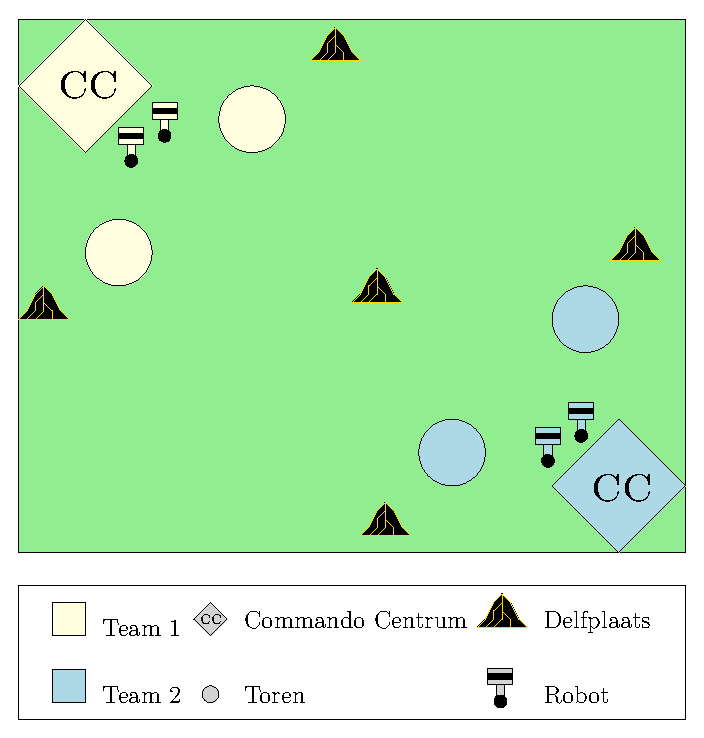
\includegraphics[width=\textwidth]{../Graphics/Map1.eps}
            \caption{Een bijna vierkant terrein met vier spelers}
            \label{fig:map1}
        \end{subfigure}\hspace{10mm}
        \begin{subfigure}{0.5\textwidth}
                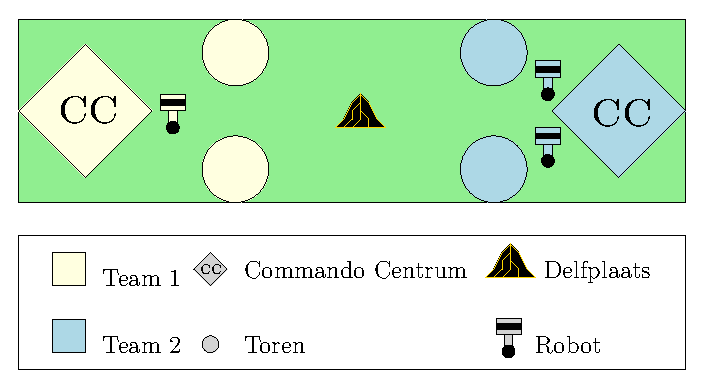
\includegraphics[width=\textwidth]{../Graphics/Map2.eps}
                \caption{Een breed terrein met drie spelers}
                \label{fig:map2}
        \end{subfigure}
        \caption{Twee verschillende beginconfiguraties van het spel}
    \end{figure}

    \subsection{Spelers}
    Een speler behoort tot \'e\'en van beide teams, spelers van een bepaald team zijn te identificeren door kleuren. De speler ziet de wereld vanuit de positie van zijn robot. Men kan de kijkrichting aanpassen, zodat deze elke willekeurige richting kan zijn. Als de kijkrichting verder naar links of rechts wordt gedraaid, draait de robot mee. De speler heeft een lasergeweer waarmee hij op andere spelers en torens kan schieten om deze te vernietigen. Het lasergeweer schiet laserstralen met een `oneindige' snelheid in de huidige kijkrichting. Bij het begin van het spel heeft de robot nog een volledig harnas. Zodra de speler wordt geraakt, wordt de conditie van het harnas slechter. Het is echter niet mogelijk dat een speler het harnas van een andere speler uit hetzelfde team beschadigt.
    \FloatBarrier
    Een speler gaat dood als zijn harnas kapot is. In dat geval zal hij na een bepaalde hoeveelheid tijd terugkeren bij het commandocentrum met een volledig harnas. Ook kan een speler gebouwen bouwen, hiervoor gebruikt hij goud uit de kas van het team. De spelers kunnen op het grondvlak bewegen met een vaste snelheid in elke richting. De enige voorwaarde hierbij is dat de spelers op de kaart blijven en niet door een gebouw lopen. Het is dus wel mogelijk dat spelers door elkaar heen kunnen lopen. De speler kijkt vanuit een derde persoon perspectief. In een derde persoon perspectief wordt de sc\`ene bekeken vanaf een punt vlak achter de speler. Het is eventueel mogelijk om dit verder uit te breiden, zodat de speler kan wisselen van derde persoon perspectief naar eerste persoon perspectief.

    \subsection{Gebouwen}
    Er zijn drie soorten gebouwen: torens, mijnen en commandocentra. Torens schieten op spelers en andere gebouwen in hun bereik. Mijnen kunnen over delfplaatsen worden gebouwd met het doel de inkomsten van een team te vergroten. In principe levert elke mijn een vaste hoeveelheid goud voor de gezamenlijke kas op. Deze hoeveelheid wordt periodiek toegevoegd aan de kas.

    Uit sommige delfplaatsen kan maar een bepaalde hoeveelheid goud worden gehaald, daarna is de delfplaats op. Dan zal de mijn over die delfplaats geen verdere bijdrage meer leveren voor de gezamenlijke kas. We staan echter ook delfplaatsen toe die een onbeperkte hoeveelheid goud bevatten. Standaard levert elke mijn hetzelfde bedrag op met dezelfde periode, maar dit kan later nog worden aangepast.

    Het commandocentrum is het belangrijkste gebouw van het team. Als dit gebouw kapot is, heeft het bijbehorende team verloren. Gebouwen kunnen door spelers worden beschoten, waardoor deze worden beschadigd. Gebouwen kunnen op geen enkele mogelijke manier hersteld worden. Optioneel zou men mechanismen in het spel kunnen toevoegen om deze gebouwen te herstellen. Alle gebouwen behoren tot \'e\'en van beide teams, deze gebouwen kunnen weer ge\"identificeerd worden door de kleur van het gebouw.

    \subsection{Verzamelbare voorwerpen}
    Er is maar \'e\'en verzamelbaar voorwerp: een muntje. E\'en of meerdere muntjes worden achtergelaten door spelers die dood gaan en torens die worden vernietigd. Een muntje heeft een bepaalde waarde in goud. De waarde van de muntjes zijn proportioneel aan de gezamenlijke kas van het team waarvan de speler is doodgegaan. Als een toren is vernietigd, dan is de waarde van de muntjes proportioneel aan de kosten van de toren. De waarde van de muntjes moet echter altijd kleiner zijn dan de kosten van de toren. Gedurende een spel moeten deze proporties vast zijn.

    Als een speler doodgaat, wordt bovendien nog de waarde van de muntjes afgetrokken van de gezamenlijke kas van die speler. Een muntje kan vervolgens opgepakt worden door alle spelers. Het muntje is dus het voedsel element in ons spel. De waarde van het muntje zal dan toegevoegd worden aan de kas van het bijbehorende team.

    \subsection{Initialisatie}
    De spelers kunnen zelf kiezen bij welk team ze gaan, onder de voorwaarde dat elk team minstens \'e\'en speler heeft. Bij de start van het spel staan alle spelers bij het commandocentrum. Zoals al eerder gezegd, hebben alle spelers dan nog een volledig harnas. Bovendien heeft elk team een zekere positieve hoeveelheid goud in de gezamenlijke kas, die voor beide teams natuurlijk gelijk moet zijn. Er kan minstens \'e\'en mijn gebouwd worden met deze hoeveelheid goud.
    \FloatBarrier

    \subsection{Gebruikersomgeving}
    \label{sec:UI}

    Via de gebruikersomgeving kan de speler de interactie met het 3D-model aangaan. De volgende componenten worden weergegeven op de gebruikersomgeving tijdens het spel:
    \begin{itemize}
    \item De hoeveelheid goud van het team, deze hoeveelheid staat achter een goudstaaf.
    \item De sterkte van het harnas, die wordt weergegeven door middel van een statusbalk.
    \item Het vizier van de speler.
    \item Een plattegrond.
    \end{itemize}

    We plaatsen het vizier van de speler altijd in het midden van het scherm. Hierdoor weet de speler dus in welke richting wordt geschoten. Voor de duidelijkheid hebben wij hier ook een figuur van gemaakt, zie figuur \ref{fig:UI}.
    \begin{figure}[H]
    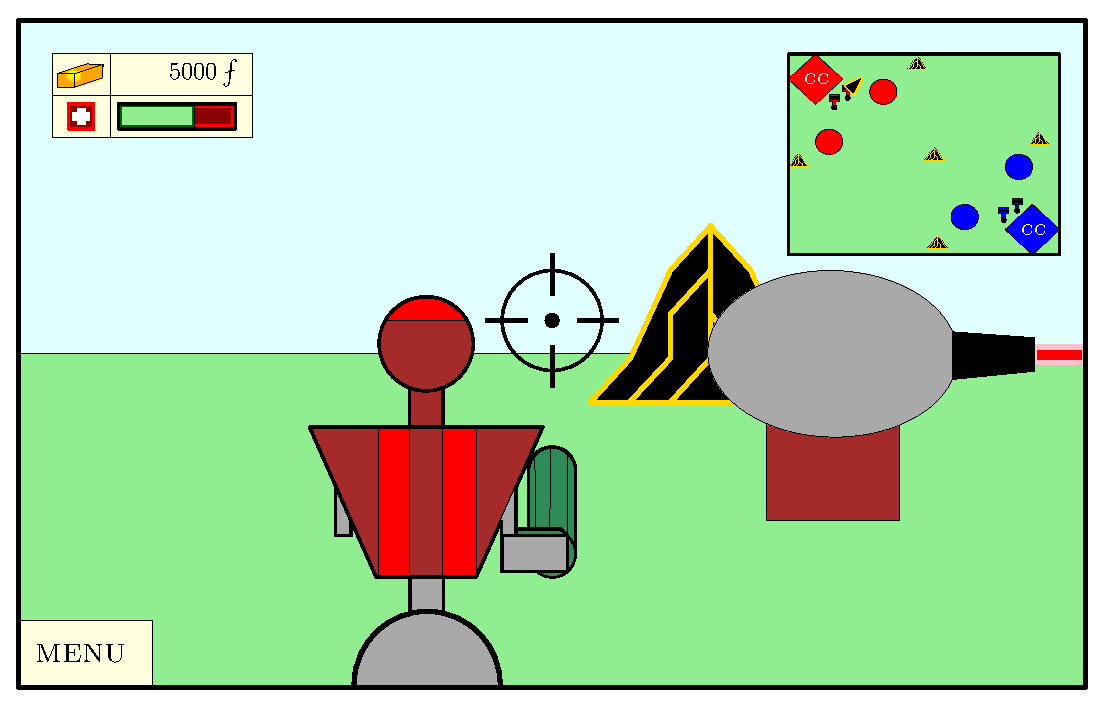
\includegraphics[width=0.9\textwidth]{../Graphics/UI.eps}
    \caption{De gebruikersomgeving tijdens het spel}
    \label{fig:UI}
    \end{figure}
    De besturing van de robot kan met de \textsc{wasd}-toetsencombinatie of door gebruik te maken van de pijltjes-toetsen. Hiervoor geven we de volgende tabel:
    \begin{table}[H]
        \small
        \centering
        \begin{tabular}{| l | l |}
        \hline
        Knop & Reactie \\ \hline
        \textsc{w} of $\uparrow$ & De robot beweegt, indien mogelijk, vooruit naar de huidige kijkrichting toe \\ \hline
        \textsc{a} of $\leftarrow$ & De robot draait naar links \\ \hline
        \textsc{s} of $\downarrow$ & De robot beweegt, indien mogelijk, achteruit van de huidige kijkrichting af \\ \hline
        \textsc{d} of $\rightarrow$ & De robot draait naar rechts \\ \hline
        \end{tabular}
        \caption{Knoppen met bijbehorende reactie}
        \label{tab:planning}
    \end{table}

    De speler kan schieten door op de muis te drukken. Een gedetailleerde beschrijving van het schieten is opgenomen in appendix \ref{app:schieten}. Door de muis naar boven of naar beneden te bewegen, kijkt de speler verder omhoog of omlaag respectievelijk. Op analoge wijze kan de speler naar links of naar rechts draaien door respectievelijk de muis naar links of naar rechts te bewegen. Merk op dat het vizier altijd in het midden van het scherm blijft. De speler ziet dit dus doordat de horizon omlaag of omhoog schuift.

    \subsection{Het neerzetten van gebouwen}
    De speler kan ook opdracht geven om op een bepaalde plek een gebouw neer te laten zetten. Om een gebouw neer te zetten moet de speler eerst op de knop \textsc{b} drukken. Dan gaat de speler in de zogenaamde \emph{bouw-modus}. Er wordt dan op de ondergrond een rooster getekend. Door middel van het vizier kan de speler een plek op het rooster aanwijzen. De speler kan dan door te klikken de opdracht geven om het gebouw te plaatsen. Op dat moment wordt de bijbehorende hoeveelheid goud uit de gezamenlijke kas gehaald. Dit kan natuurlijk alleen als de speler voldoende goud heeft.

    Indien de speler niet genoeg goud heeft, dan zal er een waarschuwing worden gegeven. Het gebouw zal dan ook niet worden geplaatst. Als de speler wel genoeg goud heeft, zal het gebouw uit de grond verrijzen. Na het neerzetten van het gebouw blijft de speler in de bouw-modus. Door nogmaals op de knop \textsc{b} te drukken gaat de speler weer uit de bouw-modus. Dit kan gezien worden in figuur \ref{fig:gebouw}.
    \begin{figure}
    \centering
    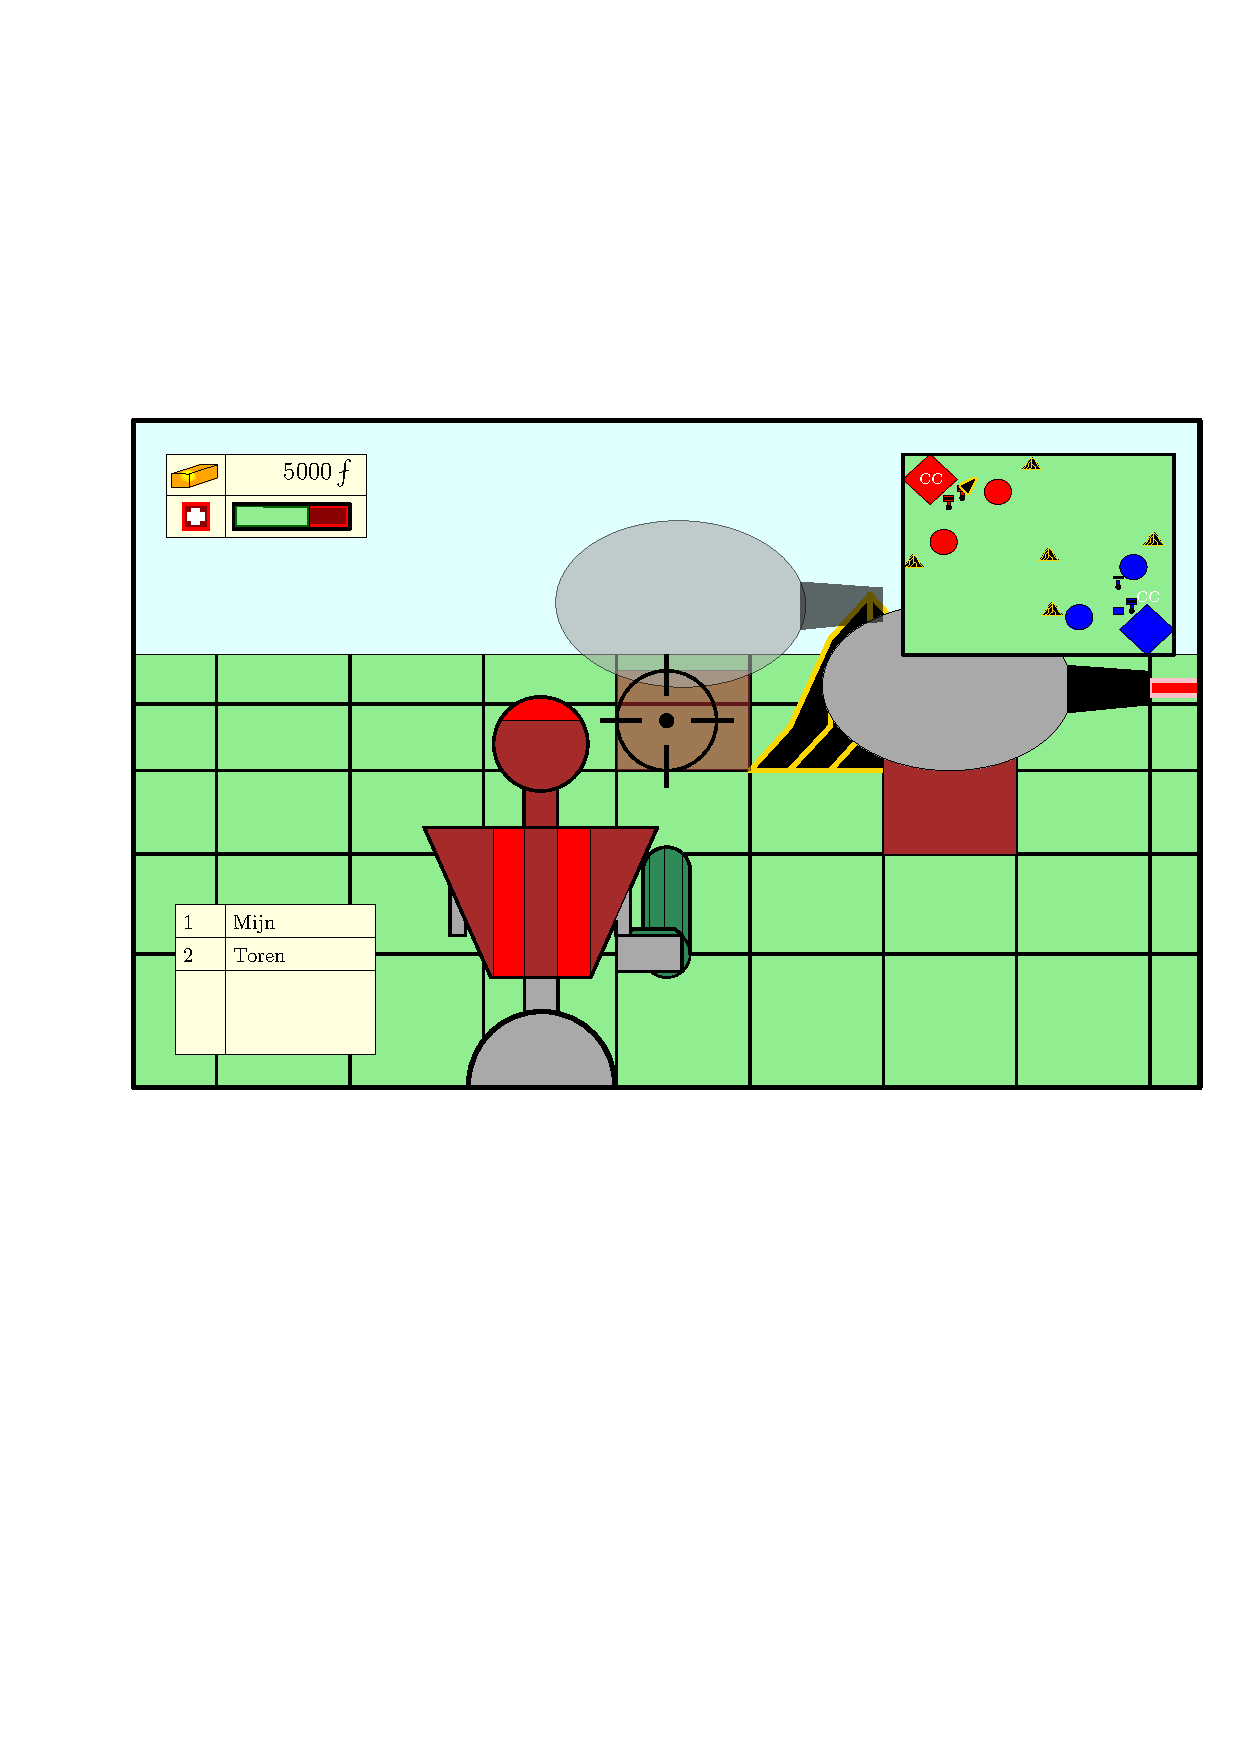
\includegraphics[width=\textwidth]{../Graphics/UI2.pdf}
    \caption{Een voorbeeld van het neerzetten van een gebouw in de gebruikersomgeving}
    \label{fig:gebouw}
    \end{figure} 
        \section{Beschrijving alternatieven}
    \label{app:alternatieven}
    Hier beschrijven we de door ons bekeken alternatieve ontwerpen voor een spel. Tijdens het brainstormen zijn we eerst de mogelijkheden gaan afbakenen door te kijken naar een aantal genres. Hierbij hebben we vooral gekeken naar persoonlijke voorkeuren. Verder hebben we natuurlijk rekening gehouden met het feit dat het spel een `voedsel' aspect moet hebben en dat het voor meerdere spelers moet zijn. Dit gaf de volgende genres:
    \begin{enumerate}
    \item[i] Strategie.
    \item[ii] Racen.
    \item[iii] First-Person Shooter.
    \item[iv] Levenssimulatie.
    \end{enumerate}
    We zullen nu elk genre dieper uitdiepen door de verschillende mogelijkheden verder in te vullen.

    \subsection{Strategie}
    We dachten bij strategie tijdens het brainstormen meteen aan het winnen van terrein als een vorm van `voedsel'. Het doel is dan om zoveel mogelijk terrein te winnen. Terrein wordt veroverd door een bepaalde tijd op een vakje te blijven staan. Verder dachten we al snel aan RTS, real-time strategie. Het idee is hier om `voedsel' te verzamelen om een leger te bouwen. Men wint dan door met dit leger de basis van de tegenstander te vernietigen.

    Via RTS kwamen we op het idee van \emph{Tower Defense}. Tower Defense wordt normaal gesproken met \'e\'en speler gespeeld. Vijandige monsters moeten dan worden tegen gehouden door torens te bouwen, die deze monsters voor jou aanvallen.

    \subsection{Racen}
    Bij een racespel dachten we aan twee alternatieven. De eerste optie was om het spelconcept van \emph{Mario Kart} ruwweg te volgen. Het doel hierbij is om zo snel mogelijk een vooraf vastgesteld aantal rondjes te rijden over een baan. Tijdens het rijden kunnen spelers power-ups verzamelen. De power-ups spelen hier dus de rol van het `voedsel'. Deze power-ups kunnen dan gebruikt worden om een voordeel te krijgen over andere spelers. Dit voordeel zou op zeer veel manieren kunnen worden gerealiseerd: zo zou een speler tijdelijk sneller kunnen gaan als gevolg van een power-up. Een andere mogelijkheid is de power-up af te kunnen schieten op andere spelers. Geraakte spelers kunnen dan worden vertraagd of tijdelijk stil komen te staan.

    Een tweede optie is dat spelers rond kunnen rijden in een grote stad. Het doel is dan om de auto's van alle andere spelers te vernietigen. Een auto van een tegenstander kan worden beschadigd door tegen de zijkant aan te rijden. Bovendien kan het spel verder worden uitgebreid, zodat de auto ook kan worden beschadigd door andere objecten.

    \subsection{First-Person Shooter}
    De First-Person Shooter is een alom bekend spelconcept. Een speler kan vrij over een gebied rondlopen. Meestal zal de speler een of ander wapen bij zich hebben. Met dit wapen kunnen andere spelers worden aangevallen. Het doel is dan om zoveel mogelijk medespelers uit te schakelen. Vaak is het zo dat een speler na een bepaalde tijd kan terugkeren in het spel, nadat die is uitgeschakeld.

    \subsection{Levenssimulatie}
    We dachten bij levenssimulatie aan een spel dat ge\"inspireerd is op het bekende spel \emph{Spore}. Ieder speler heeft in dit spel zijn eigen schepsel. Men kan zijn eigen schepsel laten groeien door andere schepsels, die niet noodzakelijk worden bestuurd door medespelers, op te eten. Het doel is dan om als enige over te blijven.

    \newpage
    \section{Motivering keuze}
    \label{app:motivering}
    In deze appendix motiveren we onze keuze uit de verschillende alternatieven in appendix \ref{app:alternatieven}. Tijdens het brainstormen was strategie meteen een van onze persoonlijke voorkeuren. Dit vonden wij allen een aantrekkelijk genre om te spelen. Het nadeel bij het veroveren van terrein is dat men al snel vastzit aan een grid. Dit is echter slechts een zeer kleine beperking. E\'en van onze verdere uitwerkingen van het genre strategie was RTS. Echter, RTS wordt al snel zeer complex om te maken, wat een groot nadeel is.

    Dit is ook de voornaamste reden dat we het simpelere Tower Defense hebben bekeken. Tower Defense is in onze mening relatief eenvoudig, maar toch aantrekkelijk om te spelen. De vraag was toen hoe Tower Defense kon worden uitgebreid tot een spel voor meerdere spelers. Het idee, dat hieruit kwam, is de basis voor het uiteindelijke spel, waarvan een korte samenvatting is uitgewerkt in het volgende hoofdstuk.

    Een racespel was ons voornaamste alternatief voor strategie. Ook dit vonden wij allen een aantrekkelijk genre om te spelen. We hadden hier, zoals al eerder besproken, ruwweg twee idee\"en: bij de eerste optie was het doel om zo snel mogelijk een vooraf bepaald aantal rondjes te rijden, bij de tweede optie was het doel om de auto's van alle andere spelers te vernietigen.

    Bij de eerste optie is er een mogelijk probleem dat power-ups, die in onze mening vitaal zijn om het spel leuk te maken, niet makkelijk kunnen worden ge\"implementeerd. Er zijn drie potenti\"ele problemen bij de tweede optie: zo is het niet duidelijk wat het `voedsel' aspect hier is. Bovendien is het zeker niet eenvoudig om te bepalen wie tegen wie aanrijdt. Als laatste is het visueel weergeven van de schade aan een auto lastig.

    Het spelconcept van First-Person Shooter hebben we niet uitgebreid bekeken tijdens het brainstormen. Ons voornaamste bezwaar was dat het zeer gecompliceerd is om te bepalen of iemand is geraakt door een kogel. Aangezien dit een zeer complex spelconcept is, willen wij dit zo simpel mogelijk houden. Daarom hebben we besloten dat spelers elkaar beschieten met lasers, die een snelheid van `oneindig' hebben. Zo kan dus direct bij het schot worden bepaald of het raak dan wel niet raak is. Dit vermijdt het probleem van bewegende objecten in de scene.

    Een groot voordeel is dat First-Person Shooters uit zichzelf al voor meerdere spelers zijn. Daarom is een deel van het First-Person Shooter concept ook opgenomen in het uiteindelijke spelconcept. Op deze manier kon het Tower Defense concept verder worden aangevuld tot een spel voor meerdere spelers: spelers kunnen elkaar aanvallen in het spel door elkaar te beschieten.

    Bij het idee van levenssimulatie werden wij ge\"inspireerd door het welbekende Spore, wat door een aantal van ons met enthousiasme is gespeeld. Er is ook een zeer duidelijk `voedsel' aspect aanwezig. Het was ons echter niet duidelijk hoe dit spel op een aantrekkelijke doch eenvoudige manier kon worden uitgebreid naar een spel voor meerdere spelers.

    \subsection{Het spel}
    Het uiteindelijke spel combineert een aantal van de eerdere idee\"en, met name Tower Defense en First-Person Shooter. We geven hier slechts een korte samenvatting van het spel. Een uitgebreide beschrijving van het spel staat in de spelspecificatie. We verdelen de spelers in twee teams. Spelers kunnen over het terrein rondlopen. Terwijl spelers rondlopen, kunnen ze torens bouwen met goud. Er zijn twee type torens: het eerste type toren kan op een mijn worden gebouwd en verzamelt extra goud. Het tweede type toren kan spelers aanvallen. Spelers kunnen andere spelers en torens aanvallen, dit is meteen ook de tweede manier om goud te verdienen. Als spelers doodgaan, komen ze een tijd later weer bij een speciaal gebouw terecht: het hoofdgebouw. Elk team heeft ook een hoofdgebouw, het doel van het spel is om het hoofdgebouw van het andere team te vernietigen.

    We hebben dus uiteindelijk gekozen voor een combinatie van de eerder genoemde spelconcepten. In onze mening is het daarmee een potentieel aantrekkelijk en innovatief spel. Het innovatieve element aan het spel is dat zowel elementen uit RTS als First-Person Shooter worden gecombineerd. Het grootste probleem is echter daarmee meteen de haalbaarheid van het spel. Elk spel moet al rekening houden met het netwerk aspect en bovendien met het gedistribueerde aspect, aangezien er geen server mag zijn tijdens het spel.  
        \section{Het ontwerp}
    % Inclusief alternatieven, motivering van keuzes, aannames en communicatieprotocol
    Nu zijn we klaar om het ontwerp van ons spel \textsc{GOTO} te bespreken. We zullen beginnen door de verschillende componenten te analyseren. Het programma is hierbij verdeeld in drie zo onafhankelijk mogelijke componenten. Wij onderscheiden de volgende componenten:
    \begin{itemize}
    \item Een component die het communiceren naar andere spelers mogelijk maakt;
	\item Het model van de sc\`ene. Denk hierbij aan de staat, locatie en grafische modellen van gebouwen, spelers en het terrein;
	\item De gebruikersomgeving die de interactie van de speler met het spel mogelijk maakt en ook het grafische model weergeeft tijdens het spel.
    \end{itemize}

    Als uitgangspunt ontwerpen wij de verschillende componenten zodanig dat elke component zo onafhankelijk mogelijk ontwikkeld kan worden.
    	
    \subsection{Protocol module}
    De protocol module is het onderdeel die het mogelijk maakt om:
	\begin{itemize}
    \item Een nieuw spel op te starten. Het spel komt dan in de zogenaamde opstart fase. Andere spelers kunnen dan aan dit spel meedoen, ze komen dan in de lobby van dat spel;
	\item De lijst van alle spellen, die nog in de opstart fase zijn, in het subnet van de computer weer te geven;
	\item Mee te doen met een bestaand spel dat nog in de opstart fase zit;
	\item Het spel te beginnen;
	\item Mutaties van de staat van het spel te ontvangen en te versturen.
	\end{itemize}
    De manier, waarop deze communicatie verloopt, is beschreven vanaf \protoref. De gebruikersomgeving kan de protocol module een opdracht geven. Deze    opdracht zal dan asynchroon worden uitgevoerd door de protocol module. Dit betekent dat het protocol uit zichzelf berichten kan ontvangen en verwerken. Door middel van threads wordt er voor gezorgd dat het protocol de taken onafhankelijk kan uitvoeren.
	
    \subsection{Het model van de sc\`ene}
    Het model van de sc\`ene vervult twee rollen. Het houdt de huidige staat van het spel bij en zorgt ervoor dat de huidige staat van het spel afgebeeld kan worden op het scherm. Het model is dus in principe een passief element, het zal niet uit zichzelf acties uitvoeren (uitzonderingen daargelaten). Een diepgaande beschrijving van het model kan gevonden worden in appendix \ref{app:klassenbeschrijving}.

    \subsection{Gebruikersomgeving}
    De gebruikersomgeving moet zowel het grafische model van het spel afbeelden op het scherm als de interactie van de speler via het toetsenbord en muis afhandelen. Ook moet de gebruikersomgeving het mogelijk maken voor de gebruiker om een spel op te starten of mee te doen aan een spel in de opstart fase.

    \subsubsection{De opzet van het spel}
    Tijdens de opzet van het spel zal de gebruikersomgeving een venster weer moeten geven met alle spellen in het subnet van de computer. De gebruiker kan dan kiezen om mee te doen aan een van deze spellen of zijn eigen spel te openen. Als de gebruiker zelf een spel opent, kunnen andere gebruikers in hetzelfde subnet ook meedoen aan dit spel. Deze spelers kunnen dan met elkaar communiceren in een lobby. Hierin kunnen zij ook aangeven of zij klaar zijn om het spel te starten. Zodra alle gebruikers hebben aangegeven dat zij klaar zijn, kan het spel worden gestart. De keuze om het spel te starten is dan aan de gebruiker, die ook het spel heeft geopend.

    \subsubsection{Tijdens het spel}
    De gebruikersomgeving zal tijdens het spel via \textsc{openGL} de lokale staat van het spel afbeelden op het scherm. Dit wordt gedaan door de \emph{render} methode van het object \emph{World} aan te roepen, die is beschreven in sectie \ref{sec:model}. De gebruikersomgeving zal daarna alleen nog menu's, mogelijke kaarten en informatie als de sterkte van het harnas en de hoeveelheid geld op het scherm moeten aangeven (zoals beschreven in het document Informele Beschrijving). Door de 2D-modus van openGL te gebruiken kan dit gemakkelijk getekend worden boven op de grafische representatie van de wereld.

    De gebruikersomgeving zal ook het model aanpassen aan de hand van de interactie van de gebruiker met de omgeving. Om dit voor elkaar te krijgen slaat
    de gebruikersomgeving alle muisbewegingen, klikken en toetsenbord aanslagen op en past het model op de bijbehorende manier aan. Een verdere uitleg van de interactie tussen de gebruikersomgeving en het model is gegeven in sectie \ref{sec:interactie}.

    \section{Onderlinge samenhang}
    \label{sec:protocol}
    De drie onderdelen, die wij hierboven beschreven hebben, moeten natuurlijk allemaal met elkaar kunnen communiceren. Deze communicatie zullen we nu beschrijven.

    \subsection{Gebruikersomgeving en protocol module tijdens de opzet van het spel}
    De gebruikersomgeving en de protocol module communiceren tijdens de opzet van het spel compleet asymmetrisch. Dat wil zeggen dat het protocol op elk moment een bericht kan sturen naar de gebruikersomgeving en ook andersom. Om dit mogelijk te maken, heeft de protocol module verschillende functies ge\"implementeerd, die aangeroepen kunnen worden door de gebruikersomgeving. Deze kunnen bijvoorbeeld gebruikt worden om een nieuw spel aan te maken of mee te doen aan een bestaand spel. Op deze manier kan de gebruikersomgeving acties van de gebruiker omzetten in een actie van het protocol: de protocol module handelt dit dan af.

    De protocol module luistert actief naar binnenkomende berichten. Aangezien het protocol real-time verplichtingen heeft, zal de module gebruik maken van meerdere threads. Zo fungeert de module los van de gebruikersomgeving. Als er een bijzondere gebeurtenis heeft plaatsgevonden, kan het protocol dit doorgeven aan de gebruikersomgeving door middel van zogenaamde \emph{call-backs}. Dit zijn methoden die de gebruikersomgeving implementeert, zodat de protocol module informatie kan doorgeven aan de gebruikersomgeving. De gebruikersomgeving zal deze informatie zodanig moeten afhandelen dat het afgebeeld kan worden op het scherm.

    Niet alle communicatie van de protocol module en de gebruikersomgeving verloopt via call-backs en methoden, sommige informatie zal de protocol module namelijk niet als een gebeurtenis doorgeven. Deze informatie wordt louter opgeslagen in de protocol module en kan de gebruikersomgeving opvragen. Denk hierbij aan de lijst van spellen op het subnet, spelers in het spel, enzovoorts. Een voorbeeld van interactie van de gebruikersomgeving en protocol module is gegeven in een \textsc{msc} in appendix \ref{app:MSCLobbyCon}.

    \subsection{Model van de sc\`ene en de gebruikersomgeving tijdens het spel}
    \label{sec:interactie}
    Het model van de sc\`ene zal niet actief communiceren met de gebruikersomgeving tijdens het spel. Dat wil zeggen dat er geen asymmetrische communicatie plaatsvindt via call-backs. De gebruikersomgeving zal aan de hand van de invoer van de gebruiker het model aanpassen. De gebruikersomgeving zal ook de grafische representatie van de staat van het spel uit het model halen. Het model maakt dit mogelijk door de beschreven \emph{render} methode in de interface \emph{object}. Het model zorgt voor enkele globale methoden die in \'e\'en keer een actie van de gebruiker kan verwerken in het model. Hierdoor hoeft de gebruikersomgeving alleen een paar globale methoden aan te roepen. Hiermee voorkomen wij dat de gebruikersomgeving veel gebruik moet maken van de structuur van het model. Zo wordt de gebruikersomgeving minder afhankelijk van de implementatie van het model.

    We hebben nu de verschillende componenten en hun onderlinge communicatie uitgediept. Een volledige beschrijving van de klassen wordt gegeven in appendix \ref{app:klassenbeschrijving}. Er is ook een bijbehorend klassediagram gemaakt. Het klassediagram is te vinden in appendix \ref{app:klassendiagram}. We zullen nu verder gaan met de beschrijving van het protocol.

    \section{De opbouw van de graaf}
    Het protocol zal een volledige graaf proberen op te bouwen. Het berichtsformaat wordt formeel gedefinieerd in appendix \ref{app:berichtsformaat}. De bijbehorende berichten zijn beschreven in appendix \ref{app:berichten}. Dit wordt gedaan tijdens de lobby fase van het spel. We weten dat er tijdens de lobby fase een server is. Elk proces probeert nu een \tcp-connectie te maken met deze server. Zodra deze \tcp-connectie is geslaagd, zal het proces een lijst teruggestuurd krijgen. Deze lijst bevat alle adressen van processen, waarmee de server nu is verbonden. Verbindingen uit de lobby fase tellen hierbij dus niet mee. Het proces is dan zelf verantwoordelijk om een \tcp-connectie aan te gaan met elk proces in deze lijst.

    Dit betekent dat op elk willekeurig moment een aanvraag voor een \tcp-connectie kan binnenkomen bij processen, die al een \tcp-connectie met de server hebben. Kortom, elk proces zal regelmatig moeten controleren op aanvragen voor een \tcp-connectie. Als de volledige graaf is opgebouwd, staan alle processen op gelijke voet. Op dat moment kan het spel beginnen.

    \section{Het protocol tijdens het spel}
    \label{sec:tijdensspel}
    De staat van het spel wordt uniek vastgelegd door de waarde van alle variabelen, inclusief de toestand van alle \tcp-connecties. Het is echter ondoenlijk om alle waarden van de variabelen voortdurend te versturen over de \tcp-connecties. Daarom zal elke speler een replica van het spel hebben. Deze replica's moeten natuurlijk zodanig worden gesynchroniseerd dat spelers er niet achterkomen dat hun replica's op kleine details tijdelijk kunnen verschillen.

    \subsection{Reliable en unreliable variabelen}
    We maken daarom onderscheid tussen twee soorten variabelen, \emph{reliable} en \emph{unreliable}. Reliable variabelen moeten gelijk zijn voor alle replica's om inconsistentie te voorkomen. Unreliable variabelen mogen wel verschillen tussen de spelers. Deze kunnen dus worden `gesimuleerd' door spelers. Om de reliable variabelen consistent te houden hebben we zogenaamde \emph{mutual exclusion} nodig. Een goed voorbeeld hiervan is het oprapen van een muntje.

    We pakken dit probleem aan door de notie van autoriteit te introduceren. Op elk moment heeft precies \'e\'en proces autoriteit. Als het proces autoriteit heeft, dan mag het proces reliable variabelen veranderen. Hiervoor wordt een bericht naar elk ander proces gestuurd. Het proces wacht dan totdat iedereen heeft teruggestuurd dat dit bericht is ontvangen. Als het proces alle wijzigingen van reliable variabelen heeft doorgegeven, krijgt een ander proces autoriteit.

    \subsection{De token ring}
    De volgende vraag is nu hoe we deze notie van autoriteit gaan verwerken in het protocol. Dit doen we door gebruik te maken van een \emph{token ring}. We bouwen tijdens de lobby fase (opstart fase) ook een ring op tussen alle processen. Dit doen we pas nadat de volledige graaf al is opgebouwd. Een mogelijke aanpak om dan een ring op te bouwen is om aan ieder proces een verschillend element uit een totaal geordend domein toe te kennen.

    We kunnen dit beschouwen als een injectieve functie $f$ van de verzameling processen $P$ naar een totaal geordende domein. Aangezien er sprake is van een totaal geordend domein, kunnen we deze waarden sorteren. Stel nu dat $P = \{ p_1, \ldots p_n\}$. Dit geeft ons een permutatie $\sigma$ zodanig dat:
    \[
    f(p_{\sigma(1)}) < f(p_{\sigma(2)}) < \ldots < f(p_{\sigma(n)})
    \]
    We verbinden nu $p_{\sigma(1)}$ met $p_{\sigma(2)}$, $p_{\sigma(2)}$ met $p_{\sigma(3)}$ enzovoorts. Bovendien verbinden we $p_{\sigma(n)}$ met $p_{\sigma(1)}$. We zijn er nu dus in geslaagd om de ring te construeren. Voor het totaal geordende domein kunnen we IP-adressen gebruiken, zodat uniciteit is gegarandeerd.

    Zodra een proces het token heeft, heeft het proces autoriteit. Het kan dan alle gewenste veranderingen van de reliable variabelen doorsturen over de volledige graaf. De andere processen zullen dan een \emph{acknowledgement} terugsturen dat dit bericht is ontvangen. Zodra alle acknowledgements van de andere processen zijn ontvangen, zal het proces de token zo snel mogelijk doorsturen naar het volgende proces in de ring. Dit zorgt ervoor dat elk proces binnen een eindige hoeveelheid tijd de token krijgt. Er is dus een zekere vorm van \emph{fairness}.

    \subsection{Simulatie}
    Sommige acties mogen ook worden uitgevoerd wanneer het desbetreffende proces niet de token heeft. Een speler mag bijvoorbeeld vrij rondlopen zonder dit te vragen aan alle andere spelers. Dit kan ervoor zorgen dat niet alle processen exact dezelfde staat hebben. Het is echter voldoende als alle processen naar dezelfde staat convergeren. We zullen dit verder toelichten aan de hand van een voorbeeld.

    Een proces zal de positie van alle andere spelers simuleren. Dit wordt gedaan met behulp van de locatie en de looprichting. De actuele locatie en looprichting van de desbetreffende speler zal periodiek over de volledige graaf worden verstuurd. Om eventuele problemen te voorkomen zou deze periode redelijk klein moeten zijn. In de tussentijd zal het proces de huidige locatie en looprichting van de speler benaderen door de speler simpelweg `verder' te laten lopen. Merk op dat op deze manier de speler ten alle tijden de baas blijft over zijn eigen locatie.

    \section{Aannamen}
    We hebben al eerder genoemd dat het \emph{Broadcast} bericht over \udp wordt gestuurd. Hier gebruiken we de broadcast functionaliteit van \udp voor. Het is dus noodzakelijk dat alle spelers zich op hetzelfde subnet bevinden. We weten dat \udp-berichten niet noodzakelijk aan hoeven te komen. We nemen echter aan dat een \udp-bericht uiteindelijk wordt ontvangen binnen een eindige hoeveelheid tijd, als de server periodiek \udp-berichten blijft versturen.

    Een speler kan dan een keuze maken tussen alle servers, waarvan een \emph{Broadcast} bericht is ontvangen. De speler gaat dan een \tcp-connectie aan met de uitgekozen server. We nemen aan dat deze \tcp-connectie succesvol wordt aangemaakt. Bovendien nemen we aan dat \tcp inderdaad voldoet aan de FIFO-eigenschap. Verder nemen we aan dat berichten over \tcp ook aankomen, eventueel nadat dit bericht een aantal keer opnieuw is verstuurd.

    Verder maken we nog een aantal simpele aannamen over de snelheid van het netwerk en de computers. De gebruikte berichten zijn allemaal zeer klein. We verwachten daarom dat er elke seconde zonder problemen 300 berichten over het netwerk kunnen worden verstuurd. Dit zou ruim voldoende moeten zijn om de replica's goede benaderingen van de werkelijke staat te laten zijn. Hiermee bedoelen we met een goede benadering dat het verschil met de werkelijke staat niet zou moeten opvallen voor de spelers.

    De helft van de RTT, oftewel de \emph{Round-Trip Time}, is een goede benadering voor hoe lang het duurt om een bericht te versturen. We gaan ervan uit dat de RTT kleiner is dan 200 ms. Deze aanname is zeker realistisch, aangezien de spelers in principe op hetzelfde subnet zitten. Vanwege deze aanname krijgen we ook een harde grens op de maximale afwijking van de replica's.
    \label{app:MSCLobbyCon} 
    
    % Aannamen verder uitwerken
    \section{Validatie van aannamen}
Voordat we de aannamen kunnen valideren, moeten we deze aannamen natuurlijk eerst identificeren. De aannamen zijn al uitgebreid besproken in het document \emph{Het ontwerp van het spel}. We zullen hier de belangrijkste punten herhalen:
\begin{enumerate}
\item[(i)] Er kunnen elke seconde 300 berichten over het netwerk worden gestuurd. Deze aanname is natuurlijk alleen realistisch als we nog de grootte van de berichten beperken. Alle gebruikte berichten in het spel zijn zeer klein. Daarom beperken we de grootte van de berichten tot 100 bytes, wat ruim voldoende is voor alle besproken berichten in het ontwerp. Hierbij is de grootte exclusief eventuele overhead van bijvoorbeeld TCP of IP.
\item[(ii)] Verder hebben we aangenomen dat de RTT, oftewel de \emph{Round-Trip Time}, kleiner is dan 200 ms. Dit betekent dus dat het niet langer duurt dan 100 ms om een bericht van speler A naar speler B te sturen.
\end{enumerate}

% Token 21 keer rond over internet.
We hebben deze aannamen uitgebreid getest. Hiertoe hebben we een apart programma geschreven. Testgegevens zijn helaas nog niet opgenomen in dit concept eindverslag, deze zullen nog komen in het uiteindelijke eindverslag.

    \section{Motivering voor de implementatie}
Nu zullen we onze keuzes bij de implementatie toelichten. Zo hebben wij ervoor gekozen om C++ te gebruiken. Daar zijn twee belangrijke redenen voor. Ten eerste is C++ snel. Dit is natuurlijk een voordeel bij het maken van een spel. Hierdoor kunnen ook mensen met relatief trage systemen het spel draaien zonder dat dit ten koste gaat van de grafische aantrekkelijkheid.

Ten tweede was er nog het educatieve aspect. Een deel van de groep was namelijk nog niet bekend met C++ aan het begin van het project. Deze groepsleden leren hiermee een nieuwe programmeertaal naast Java. Het is altijd handig om kennis te hebben van verschillende programmeertalen.

Verder gebruiken we \emph{WxWidgets} bij de implementatie. De reden hiervoor is de grote diversiteit aan \emph{Operating Systems}: we gebruiken zowel Windows, Mac en Linux. Een groot voordeel van WxWidgets is dat het op al deze Operating Systems werkt. Ook gebruiken we nog \emph{Freeglut} en \emph{OpenGL}. Freeglut is een open source alternatief voor GLUT. Het voordeel van Freeglut is dat een aantal bugs in GLUT zijn verholpen in Freeglut.

Als laatste noemen we nog \emph{Autodesk 3ds Max}. Dit programma is gemaakt voor het modelleren van de sc\`ene. Hierin zijn alle textures en modellen gemaakt. Daarbij hebben we nog \emph{lib3ds} gebruikt om de textures en modellen in te laden.

    \section{Conclusie}
    % Met daarin reflectie over het verloop van het project en het groepsproces daarbij
    % Misschien ster weglaten/alles bereikt?
    We zijn erin geslaagd om een interactief, gedistribueerd 3D-spel te ontwikkelen. Dit spel voldoet aan de door ons gegeven specificatie van het spel op een kleine wijziging na. We hebben besloten om de speler rechts van het vizier te plaatsen. Daardoor staat het lasergeweer van de speler aan dezelfde kant als het vizier. Dit maakt het schieten intu�tiever in onze mening.

    Verder zijn er nog een aantal extra's ge\"implementeerd. Zo wordt er een plattegrond van de wereld op het scherm getoond: dit was een van de mogelijke uitbreidingen van het spel genoemd in de specificatie. Tijdens het spel is het ook nog mogelijk om net als in de lobby met andere spelers te \emph{chatten}. Bovendien zijn er nog verscheidene aspecten van de ster ge\"implementeerd. Spelers kunnen tijdens het spel nog meedoen of het spel onverwachts verlaten.

    \section{Evaluatie}
    % Welke wijzigingen? Geweer?
    % Script taal?
    Achteraf bezien was het netwerk aspect het grootste obstakel voor ons. Dit hadden wij van tevoren ook al verwacht. Dit is dan ook de reden dat we hier al zeer vroeg mee zijn begonnen: in de ori�ntatiefase zijn we al bezig geweest met het maken van een \emph{chatprogramma}. Voor de implementatie van het protocol zijn verschillende testprogramma's gemaakt, die zeer nuttig zijn gebleken. Door deze testprogramma's konden we effici\"ent fouten opsporen in de implementatie van het protocol. Goede planning en testen zijn hier van groot belang geweest. 
    
    Een ander obstakel voor ons was de complexiteit van het spel. We waren zelf enthousiast over ons spel. Hierdoor is onze specificatie vrij uitgebreid geworden. Een ander gevolg hiervan is dat er relatief veel tijd aan de implementatie is besteed, voor een groot deel ook buiten de OGO-tijden. Door hard werk en strakke planning hebben we uiteindelijk het door ons beoogde spel kunnen ontwikkelen.
    
    De samenwerking in de groep is goed verlopen. Iedereen in deze groep had ongeveer evenveel ervaring met programmeren. Echter, C++ was nieuw voor een aantal groepsleden. Dit was echter nauwelijks een probleem. Bij het begin van de implementatie zijn er verschillende groepen gemaakt. Hierbij is ervoor gezorgd dat er minstens \'e\'en groepslid al ervaring had met C++. Al snel werd deze nieuwe programmeertaal opgepikt door de andere groepsleden. Later tijdens de implementatiefase was deze groepsindeling ook niet meer nodig.

    \section{Literatuurlijst}
    \newpage

    \appendix
    
    % Nog geen verwijzing naar deze appendix
    \section{Begrippenlijst}
injectief\\
permutatie\\
totale ordening\\
    \newpage

    \section{Schieten met het lasergeweer}
\label{app:schieten}
Men kan opmerken uit figuur \ref{fig:UI} dat de schietrichting niet meteen duidelijk uit de gebruikersomgeving wordt. Immers, het vizier wordt niet op hetzelfde punt als het wapen op het scherm afgebeeld. Aangezien het vizier eenvoudiger is om mee te richten dan het wapen, wordt bij het schieten een laserstraal afgevuurd vanuit het wapen naar het punt waar het vizier op gericht staat. Dit is te zien in figuur \ref{fig:COL}. Als het vizier niet op een object gericht staat, dan zal, bij het schieten, de laserstraal uit het wapen afgevuurd worden in de kijkrichting.

\begin{figure}[H]
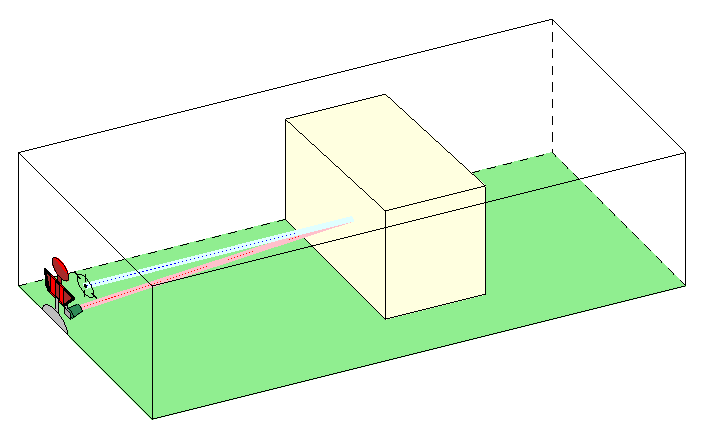
\includegraphics[width=0.9\textwidth]{../Graphics/Collision.eps}
\caption{Een voorbeeld van het schieten van het wapen, de blauwe lijn is niet zichtbaar tijdens het spelen}
\label{fig:COL}
\end{figure}

Een probleem ontstaat wanneer er een object de laserstraal vanaf het wapen naar het punt, waar het vizier op gericht staat, blokkeert. Het object zou dan geraakt moeten worden en niet het punt waar het vizier op gericht staat. Er zijn twee manieren om dit op te lossen, men kan zeggen dat de laser altijd het punt van de vizier raakt. Dit is makkelijker te implementeren, aangezien we maar \'e\'en keer hoeven te bepalen waar een lijn een object raakt. Dit is te zien in figuur \ref{fig:COL2}. Een andere oplossing is dat in dit geval de laser alleen het object, dat in de weg staat, raakt. Dit is natuurlijk realistischer, maar minder makkelijk te implementeren. Dit is te zien in figuur \ref{fig:COL3}. In eerste instantie kiezen wij voor de eerste methode. Echter, indien de tijd ons de mogelijkheid gunt om de tweede oplossing te kunnen implementeren, zullen wij de tweede oplossing implementeren.
\FloatBarrier
\begin{figure}[H]
\begin{subfigure}{0.45\textwidth}
\centering
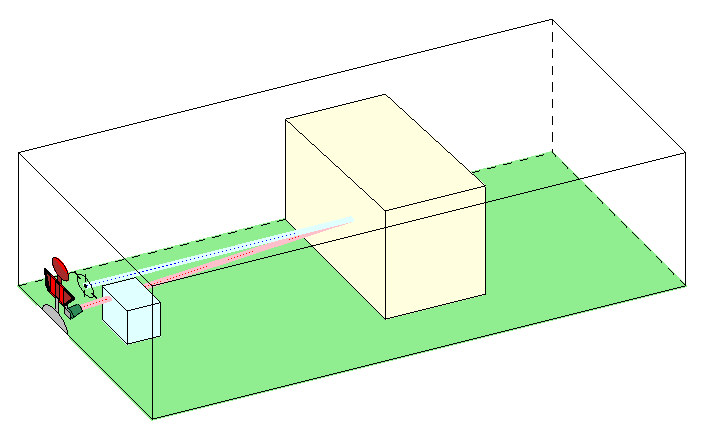
\includegraphics[width=\textwidth]{../Graphics/Collision2.eps}
\caption{De laser komt altijd aan op het punt aangewezen door het vizier}
\label{fig:COL2}
\end{subfigure}
\begin{subfigure}{0.45\textwidth}
\centering
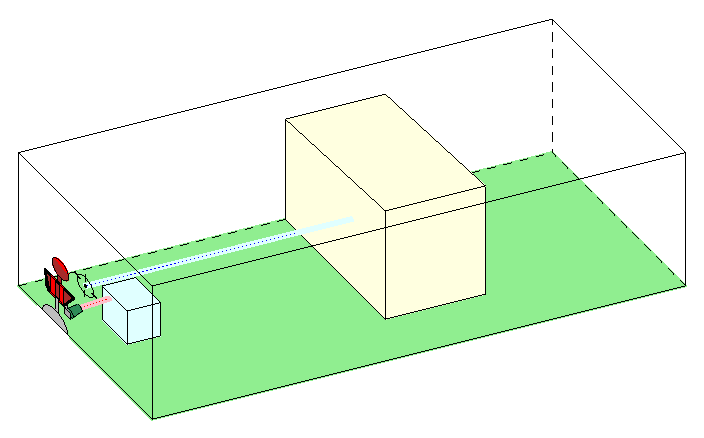
\includegraphics[width=\textwidth]{../Graphics/Collision3.eps}
\caption{De laser stopt zodra hij een ander object raakt}
\label{fig:COL3}
\end{subfigure}
\caption{Oplossingen voor de problemen bij het schieten}
\end{figure}
    \newpage
    
    \section{Optioneel}
\label{app:optioneel}
Hier bespreken we onze plannen voor uitbreiding van het spel. De volgende idee\"en zouden wij graag extra implementeren. De idee\"en zijn gesorteerd op aflopende volgorde van belangrijkheid.

\begin{itemize}
  \item Extra goud, de gezamenlijke kas wordt periodiek met een vaste hoeveelheid verhoogd. Dit is dan additief met eventuele mijnen. Wij verwachten dat dit weinig tijd kost.
  \item Oorlogsmist, de robots hebben een beperkt zichtveld. Dit voorkomt dat spelers vanaf hun commandocentrum alle activiteiten van de tegenstanders kunnen zien. Wij denken dat dit weinig tijd kost.
  \item Plattegrond, zodat spelers een globaal overzicht krijgen van wat er op de kaart gebeurt. Dit kan eventueel ook weer met een oorlogsmist zijn, zodat de spelers alleen een gedeelte van het plattegrond kunnen zien, waar teamgenoten in de buurt staan. Wij vermoeden dat dit niet veel tijd kost.
  \item Muren, als een extra type gebouw. Onze bedoeling hierbij is dat deze muren relatief goedkoop zijn om te bouwen. Dit geeft een team meer opties om hun commandocentrum of delfplaatsen te beschermen. Bovendien geeft het de extra mogelijkheid om een veilige plek te cre\"eren, waarvandaan tegenstanders aangevallen kunnen worden. Wij voorzien dat dit een kleine hoeveelheid tijd kost.
  \item Ontwikkelingen, de spelers krijgen ontwikkelingspunten tijdens het spel. Deze kunnen worden verdiend door het uitschakelen van spelers, werkers, infanterie en het vernietigen van gebouwen. Werkers en infanterie worden uitgelegd in de volgende twee idee\"en. Hiermee kunnen de spelers bijvoorbeeld de eigenschappen van hun robot verbeteren, zoals de snelheid van lopen en hoe sterk het harnas is. Ook is het mogelijk om sterkere wapens te kopen. Wij denken dat dit veel tijd kost, aangezien een `winkel' gemaakt moet worden waar deze punten gespendeerd kunnen worden. Ook moeten de eigenschappen van een speler dynamisch gemaakt worden.
  \item Werkers, dit zijn computergestuurde robots. Zodra een speler daartoe opdracht geeft, komen werkers uit het commandocentrum van het bijbehorende team om een gebouw neer te zetten. Dit vervangt de oude mogelijkheid van spelers om te bouwen. Een gevolg van deze aanpassing is dat het langer duurt om een gebouw te bouwen als de afstand van de bouwplaats tot het commandocentrum groter is. Bovendien wordt het mogelijk om het bouwen van het andere team te vertragen door de werkers uit te schakelen. Dit kost heel veel tijd, aangezien de werkers gedistribueerd bestuurd worden. Hiervoor is dus een soort gedistribueerde kunstmatige intelligentie nodig. Dit is een uitdaging. Merk ook op, dat deze computergestuurde robots niet door de gebouwen horen te lopen, waardoor deze kunstmatige intelligentie totaal niet triviaal is.
  \item Infanterie, ook dit zijn computergestuurde robots. Deze kunnen door spelers worden gekocht, vanaf het commandocentrum lopen ze naar gebouwen van het andere team om deze gebouwen aan te vallen. Dit kost nog meer tijd dan de werkers, aangezien de infanterie niet tussen twee vaste punten zich moeten verplaatsen, maar ook gebouwen moeten kunnen aanvallen.
\end{itemize} 
    \newpage

        \section{Gedetailleerde klassenbeschrijving}
    \label{app:klassenbeschrijving}
    We zullen hier de verschillende componenten verder uitdiepen aan de hand van een klassediagram. Het klassediagram bespreken we \emph{top-down}. Het klassediagram zelf is toegevoegd in appendix \ref{app:klassendiagram}. Een aantal basisklassen, zoals $Point2d, Point3d$ en $Vector3d$, zijn hierin voor de overzichtelijkheid niet aangegeven. We maken bovendien de afspraak dat de types $Percentage/Power/Time/Duration$ vrij kunnen worden gebruikt. Deze kunnen bijvoorbeeld \emph{Reals} of \emph{Integers} zijn, afhankelijk van de implementatie. We zijn nu klaar om de gebruikte interfaces te bespreken.

    \subsection{Interfaces}
    Er zijn twee interfaces in het klassendiagram: de zogenaamde $Object$ interface en $BoundingObject$ interface. We geven het implementeren van een interface aan door $\langle\langle$ interface naam $\rangle \rangle$ voor de naam van de klasse, die de interface implementeert.  De klasse Object bevat een aantal standaard attributen om de conversie tussen globale en lokale co\"ordinaten te bewerkstelligen. Dit zijn $origin, yaw, patch$ en $roll$. Hier zijn de hoeken yaw, pitch en roll in graden tussen 0 en 360. 0 is in dit geval inclusief, 360 is exclusief.

    Bovendien bevat Object nog het attribuut $children$, dit is een array van Objects. De reden hiervoor is dat dit hi\"erarchisch modelleren mogelijk maakt. Vervolgens bevat Object nog een aantal methoden: $draw, render, prerender$ en $postrender$. De prerender methode zorgt voor de transformatie van globale co\"ordinaten naar lokale co\"ordinaten. De postrender methode zorgt voor de transformatie van lokale co\"ordinaten naar globale co\"ordinaten.

    De draw methode zorgt voor het tekenen zelf. Deze methode is natuurlijk abstract gemaakt. De render methode combineert alle voorgaande methoden: het roept eerst prerender aan. Vervolgens wordt draw aangeroepen. Daarna wordt ook de draw functie van de Objects in de children array aangeroepen. Als laatste wordt nog postrender aangeroepen.

    De interface BoundingObject is een subklasse van Object. De aard van deze type objecten is zodanig dat ze begrensd zijn. Hier hoort dus een corresponderende \emph{bounding box} bij. De bounding box staat in het attribuut bBox van het type BoundingBox. Ook in dit geval geldt dat de klasse BoundingBox niet in het klassendiagram is opgenomen voor de overzichtelijkheid.

    De bounding box is niet alleen handig voor het tekenen. Het is namelijk ook mogelijk met deze bounding box te testen voor \emph{collisions}. Hier wordt getest of er een collision plaatsvindt van het object met de lijn gegeven door het startpunt origin en met richting direction. Het object zelf of een van de children wordt teruggeven in het geval van een collision. Als er geen collision is, dan zullen we \emph{null} teruggeven. Dit kan bijvoorbeeld gebruikt worden bij het schieten.

    \subsection{Model van de sc\`ene}
    \label{sec:model}
    We zijn nu klaar om de klassen, die worden gebruikt om de sc\`ene te modelleren, te bespreken.  Al deze klassen implementeren de interface BoundedObject. Merk op dat de klasse Object dus niet gebruikt wordt, behalve dat BoundedObject een subklasse hiervan is. Deze klasse kan echter nuttig zijn voor verdere uitbreiding van het spel. We beginnen met de $World$ klasse. Deze bevat een attribuut $homePlayer$ van het type $Player$. Dit attribuut wordt gebruikt om de speler zelf te identificeren.

    De $walkHomePlayer$ wordt gebruikt door de speler om rond te lopen door de wereld. Er wordt dan periodiek een bericht naar alle andere spelers gestuurd om dit door te geven. Verder wordt de $walk$ functie van Player aangeroepen, deze functie wordt verderop nog besproken. De $yesno$ boolean wordt gebruikt om aan te geven of de speler moet lopen of stoppen met lopen. De $shootHomePlayer$ heeft een vergelijkbare interpretatie.

    De $buildBuilding$ wordt gebruikt door de speler om een nieuw gebouw neer te zetten. Hiervoor moet natuurlijk een punt worden aangegeven op de grond en het gewenste gebouw. Het gewenste gebouw is dan van het type $Building$. Als laatste is er nog de functie $pickup$. Deze wordt gebruikt als een speler een object, zoals een muntje, opraapt. Merk op dat dit niet noodzakelijk de speler zelf hoeft te zijn. Opraapbare objecten zijn van het type $Droppable$.

    \subsubsection{Het terrein}
    $World$ heeft een $Terrain$, die het terrein van de sc\`ene voorstelt. Het terrein wordt gemodelleerd door een grid. De methode $groundCollision$ wordt gebruikt bij het bouwen van een gebouw. In deze methode wordt berekend welke cel van de grid is aangeklikt. Merk op dat de cellen van de grid worden aangeklikt met behulp van het vizier en dat het vizier altijd in de huidige kijkrichting staat. Voor groundCollision kan dus de huidige locatie en kijkrichting worden gebruikt.

    De methode $getHeight$ geeft de hoogte van het terrein voor een zekere cel terug. Op dit moment is ons terrein in principe nog vlak, maar dit willen we later nog uitbreiden. Als we het terrein hoogte willen geven, is een mogelijke optie om dit in de grid op te slaan. Aangezien het terrein nu nog vlak is, is dit nog niet opgenomen in het klassendiagram: hiervoor is slechts een simpele en kleine uitbreiding nodig.

    Terrain heeft een array van Droppables en een matrix van $Structures$. Droppable stelt een opraapbaar object voor: dat is nu alleen nog een muntje. Een opraapbaar object heeft een zekere waarde. Bovendien zal een opraapbaar object na een zekere tijd verdwijnen, hiervoor is het attribuut $dieTime$ van het type $Time$. Als laatste is er nog de methode $onPickup$. Deze methode werkt de staat van World bij na de actie die is veroorzaakt door het oppakken van een Droppable. Dus in het geval van een muntje wordt de hoeveelheid goud van het team verhoogd.

    De klasse Structure is abstract: de klassen Mine en Building zijn de subklassen. In de klasse Mine wordt opgeslagen hoeveel inkomen deze mijn genereert in een zekere periode. Deze periode is vast voor alle mijnen. Hiervoor kunnen we dus een constante defini\"eren. De klasse Building is ook weer abstract. Een Building heeft altijd \'e\'en corresponderend team. Het heeft de attributen $cost, income, buildTime, buildDuration, attackPower$ en $health$.

    Het attribuut $cost$ staat voor de totale kosten van het gebouw. $Income$ representeert het inkomen dat het gebouw genereert. Ook hier geldt dat de tijdseenheid vast is. $BuildTime$ representeert het moment waarop de speler de opdracht heeft gegeven het gebouw neer te zetten, $BuildDuration$ vertelt hoelang het bouwen duurt. Dit wordt gebruikt door de animatie van het gebouw. Het wordt verder gebruikt om te bepalen wanneer het neerzetten van het gebouw voltooid is.

    $AttackPower$ geeft aan hoe ernstig het harnas wordt beschadigd, als het gebouw een speler neerschiet. $Health$ geeft de sterkte van het gebouw aan: als de health nul wordt, gaat het gebouw kapot. We merken op dat de attributen $income$ en attackPower geen betekenis hebben voor alle gebouwen. Zo heeft attackPower geen betekenis voor de resourceMine. Als dit het geval is, zal altijd de waarde 0 moeten worden gekozen voor dit attribuut.

    De klasse $ResourceMine, DefenseTower$ en $HQ$ zijn subklassen van $Building$. Een ResourceMine is het gebouw dat over een $Mine$ kan worden geplaatst. Mine staat dus voor de delfplaats en ResourceMine voor de mijn. Een Mine hoeft dus in principe niet van een team te zijn, terwijl een ResourceMine dat altijd zal zijn.

    \subsubsection{De speler en teams}
    World heeft in principe twee $Teams$, deze klasse representeert de verschillende teams. Later kunnen we dit nog uitbreiden naar meer dan twee teams. Elk team heeft een zekere hoeveelheid goud in de kas. Dit wordt opgeslagen in het attribuut resources. Bovendien heeft Team een array van $Players$. Hierin staan natuurlijk de spelers van dat team.

    De klasse Player modelleert een speler in het spel. In het attribuut $health$ wordt de sterkte van het harnas opgeslagen. Het attribuut $lastShoot$ representeert het laatste moment, waarop de speler heeft geschoten. Hierdoor kunnen we het spel uitbreiden, zodat de speler pas weer kan schieten na een zekere \emph{cooldown} periode. De methode $fireLaser$ verzorgt de animatie bij het schieten. Hiervoor wordt de klasse $Laserbeam$ gebruikt: deze klasse heeft een $fireTime$ en $fireDuration$. De fireTime is het moment van vuren. De fireDuration bepaalt dan hoe lang de animatie van het schot duurt. De methode $walk$ in Player zorgt voor de animatie als de speler loopt. Het $connectie$ attribuut maakt het mogelijk voor de $communicator$ klasse om de bijbehorende connectie van een speler op te kunnen vragen.

    \subsubsection{De camera}
    Als laatste heeft de World nog een $Camera$. We laten het nog open voor de implementatie welke attributen worden gebruikt om de camera te representeren. De klasse $Camera$ is een abstracte klasse. Een implementatie van $Camera$ heeft dus de verplichting dat een speler vanuit het juiste punt in de juiste richting kijkt. In principe implementeren wij camera alleen door de klasse PlayerCamera: deze camera bekijkt de wereld vanuit een derde persoonsperspectief. Andere implementaties zijn later nog mogelijk.

    \subsection{Statische objecten}
    Er is nog \'e\'en cruciaal statisch object voor de implementatie van het spel, waarvan de functies door alle andere klassen kunnen worden gebruikt. Dit is de klasse $Communicator$, die de communicatie met andere spelers verzorgt. Een uitgebreide beschrijving van het protocol begint bij \protoref. Met een boolean in deze klasse wordt aangegeven of dit proces de token heeft. Verder wordt opgeslagen wanneer de token voor het laatst is ontvangen. Hiervoor gebruiken we het type Date, die de huidige tijd representeert.

    De klasse Communicator maakt gebruik van de klasse $Message$. De klasse Message representeert het bericht dat moet worden verzonden. Het heeft een attribuut type, die het soort bericht aangeeft. Dit attribuut is van het type $MessageType$, dat voor de overzichtelijkheid is weggelaten uit het klassediagram. MessageType is immers een simpele enumeratie.

    Verder heeft Message nog een boolean $requiresToken$, die aangeeft of de token vereist is om dit soort bericht te mogen versturen. De token wordt gebruikt voor mutual exclusion. Als laatste heeft het message nog een array van argumenten. Het type $Argument$ hangt af van de implementatie, hiervoor kan bijvoorbeeld string of array van bytes worden gekozen. Verder zijn er nog de methoden $addInteger, addReal, addString, addIntegers$ en $addReals$. Deze methoden voegen de type in de naam van de methode toe aan het bericht.

    De methode $broadcastMessage$ stuurt een $message$ naar elke speler die deelneemt aan het spel. Als het bericht een token nodig heeft ($requiresToken = True$) dan wordt het bericht alleen verstuurd als Communicator ook het token heeft ($hasToken = True$). In het geval dat het bericht geen token nodig heeft, wordt het bericht meteen verstuurd. Als het bericht een token nodig heeft en de communicator heeft geen token, dan wordt het bericht niet verstuurd. Dan retourneert de methode ook false: later kan nog een keer worden geprobeerd. In het geval dat het bericht wel wordt verstuurd, dan retourneert de methode true.

    Door middel van de methode $lockToken$ kan men afdwingen dat de token niet meer vrijgegeven wordt totdat $unlockToken$ wordt aangeroepen. De methode heeft \'e\'en parameter $BlockingWait$. Deze parameter geeft aan of de functie moet wachten totdat de communicator de token heeft of direct moet stoppen als de communicator de token niet heeft. Als de communicator niet kan locken omdat de token er nog niet is, retourneert de methode $false$. In elk ander geval wordt $true$ geretourneerd.

    De methode $broadcastTeamMessage$ doet hetzelfde als $broadcastMessage$ behalve dat deze alleen berichten verstuurd naar spelers die in het team $t$ zitten.
    \newpage

    \section{Klassendiagrammen in UML}
    \label{app:klassendiagram}
    
    \subsection{Interfaces}
    \begin{figure}[h]
    \centering
    	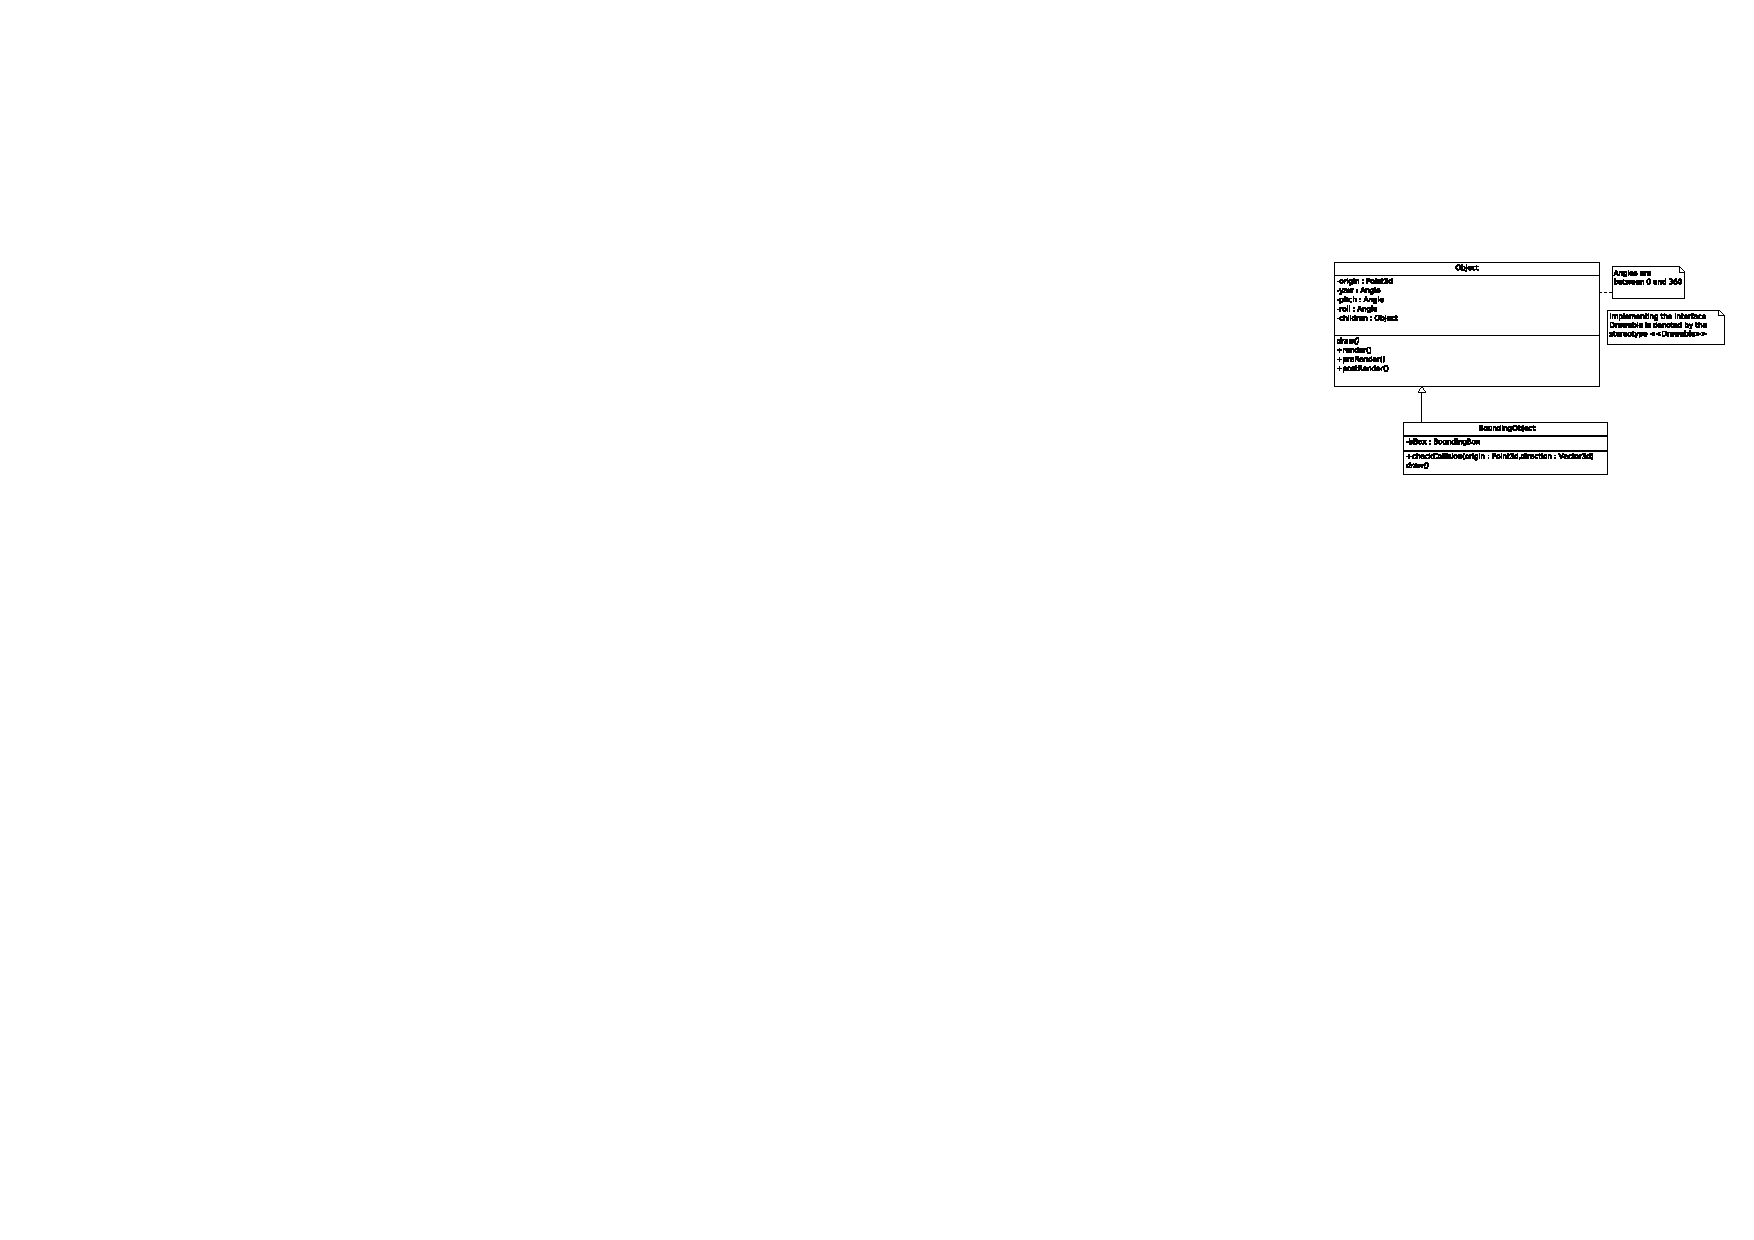
\includegraphics[width=0.9\textwidth]{../Class-diagram/Interfaces.pdf}
    	\caption{De verscheidene interfaces die ge\"implementeerd worden door klassen in het model van de sc\`ene.}
    \end{figure}\FloatBarrier    \label{app:Interfaces}
    \begin{samepage}
    
    \subsection{Communicatie klassen} \begin{figure}[h]
        \centering  	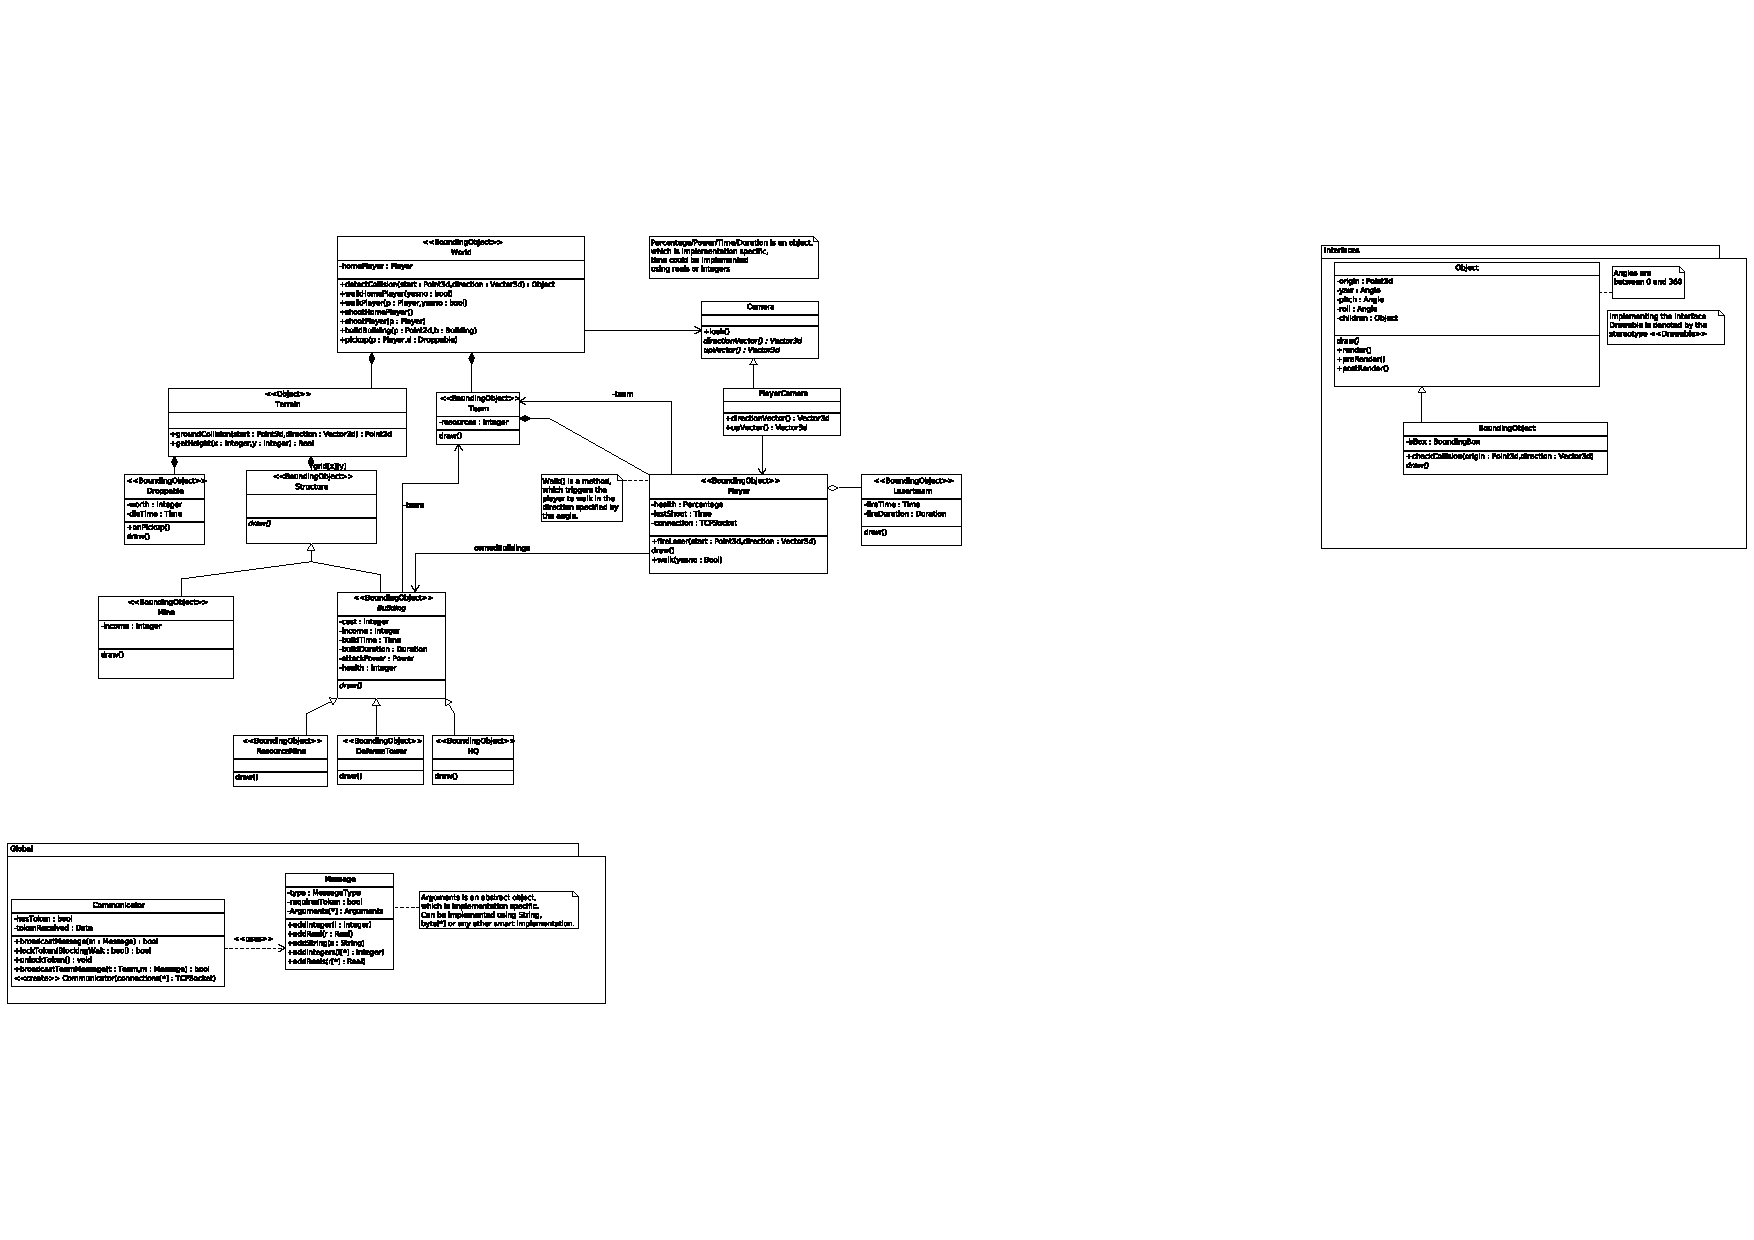
\includegraphics[width=1.05\textwidth]{../Class-diagram/NetCommunication.pdf}
	\caption{De globale klasse die methoden verschaft om te kunnen communiceren met de medespelers.}
    \end{figure}
    \label{app:Comm}
    \end{samepage}
    \FloatBarrier
    \newpage
    
    \subsection{Klassendiagram voor de sc\`ene}
    \begin{figure}[h]
        \centering
    	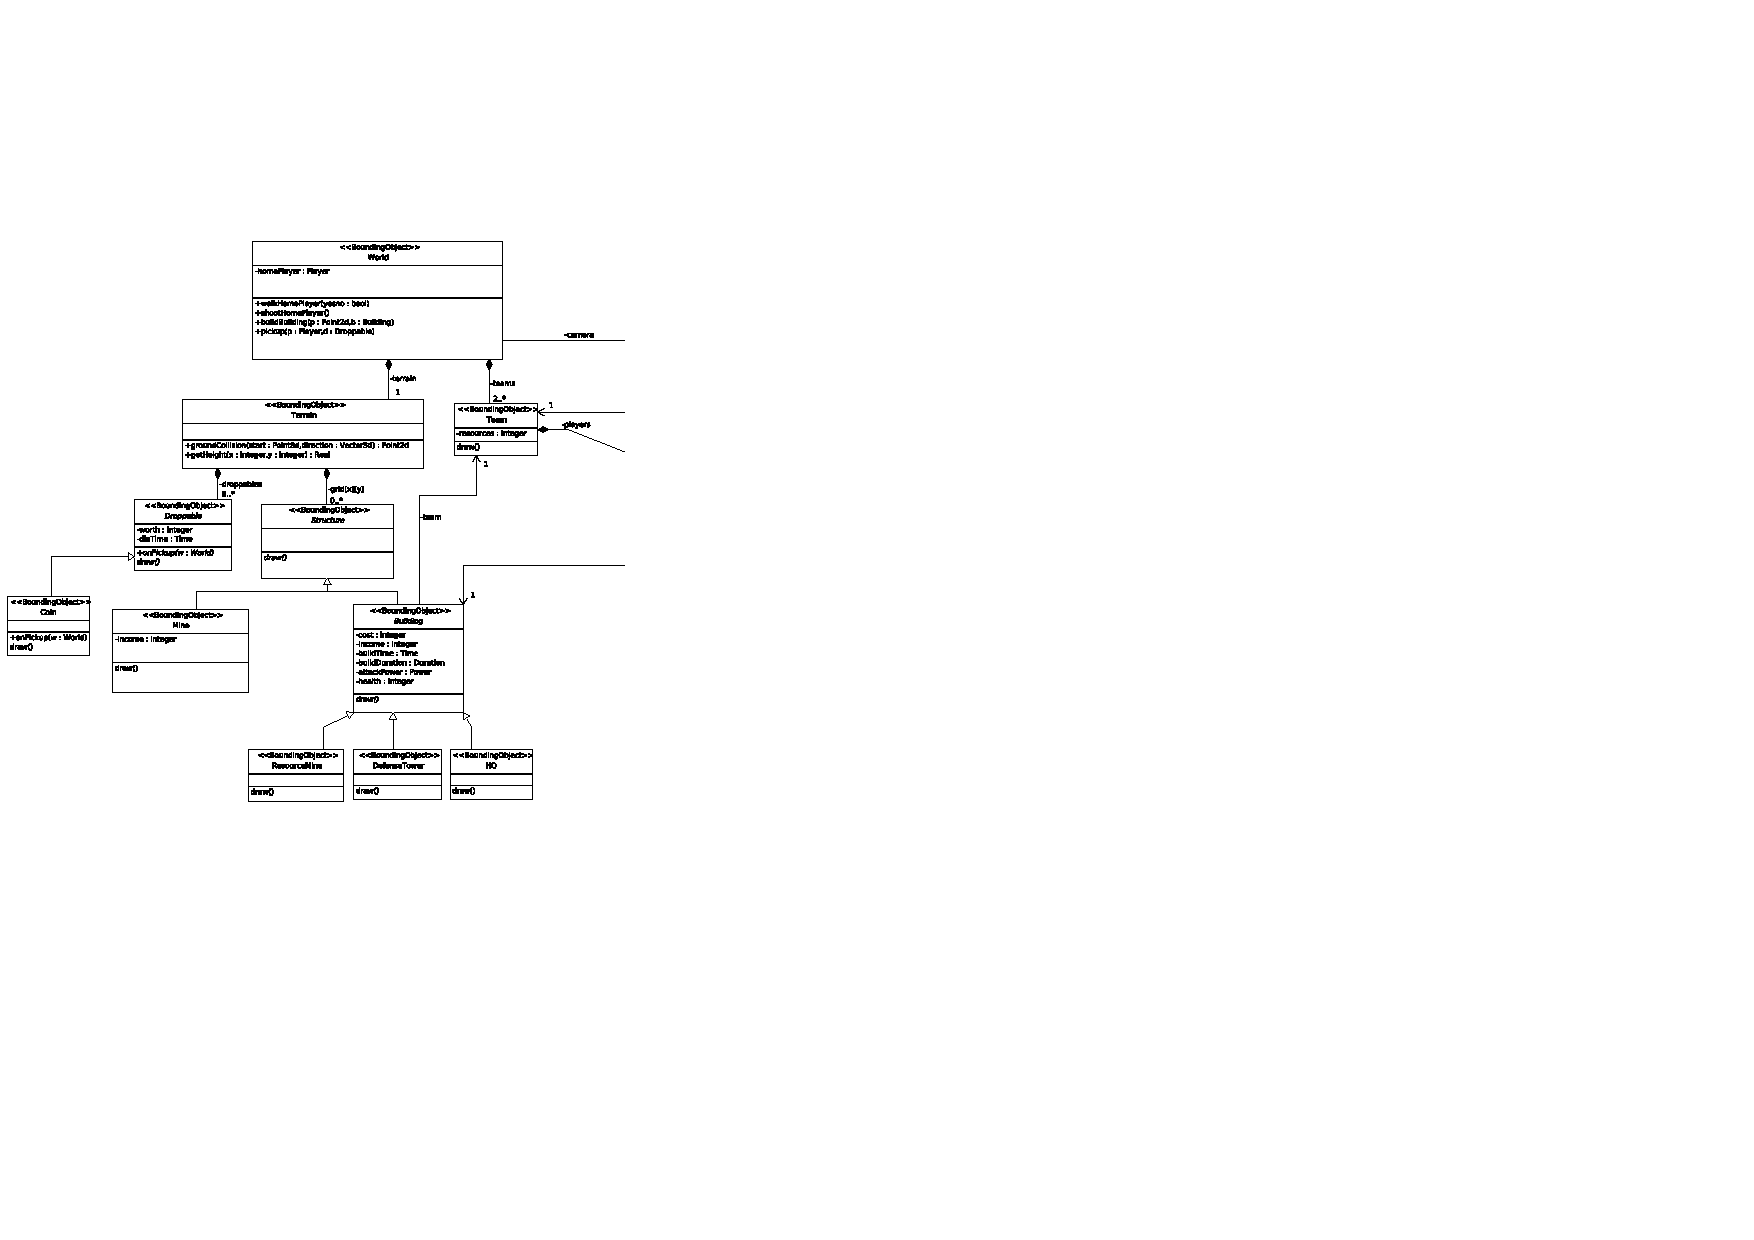
\includegraphics[height=0.72\textheight]{../Class-diagram/ClassDiagram1.pdf}
	\caption{Het klassendiagram voor het model van de sc\`ene.}
    \end{figure}
    
    \label{app:Scene}
    \FloatBarrier
    \newpage
     \ \\[5mm]
    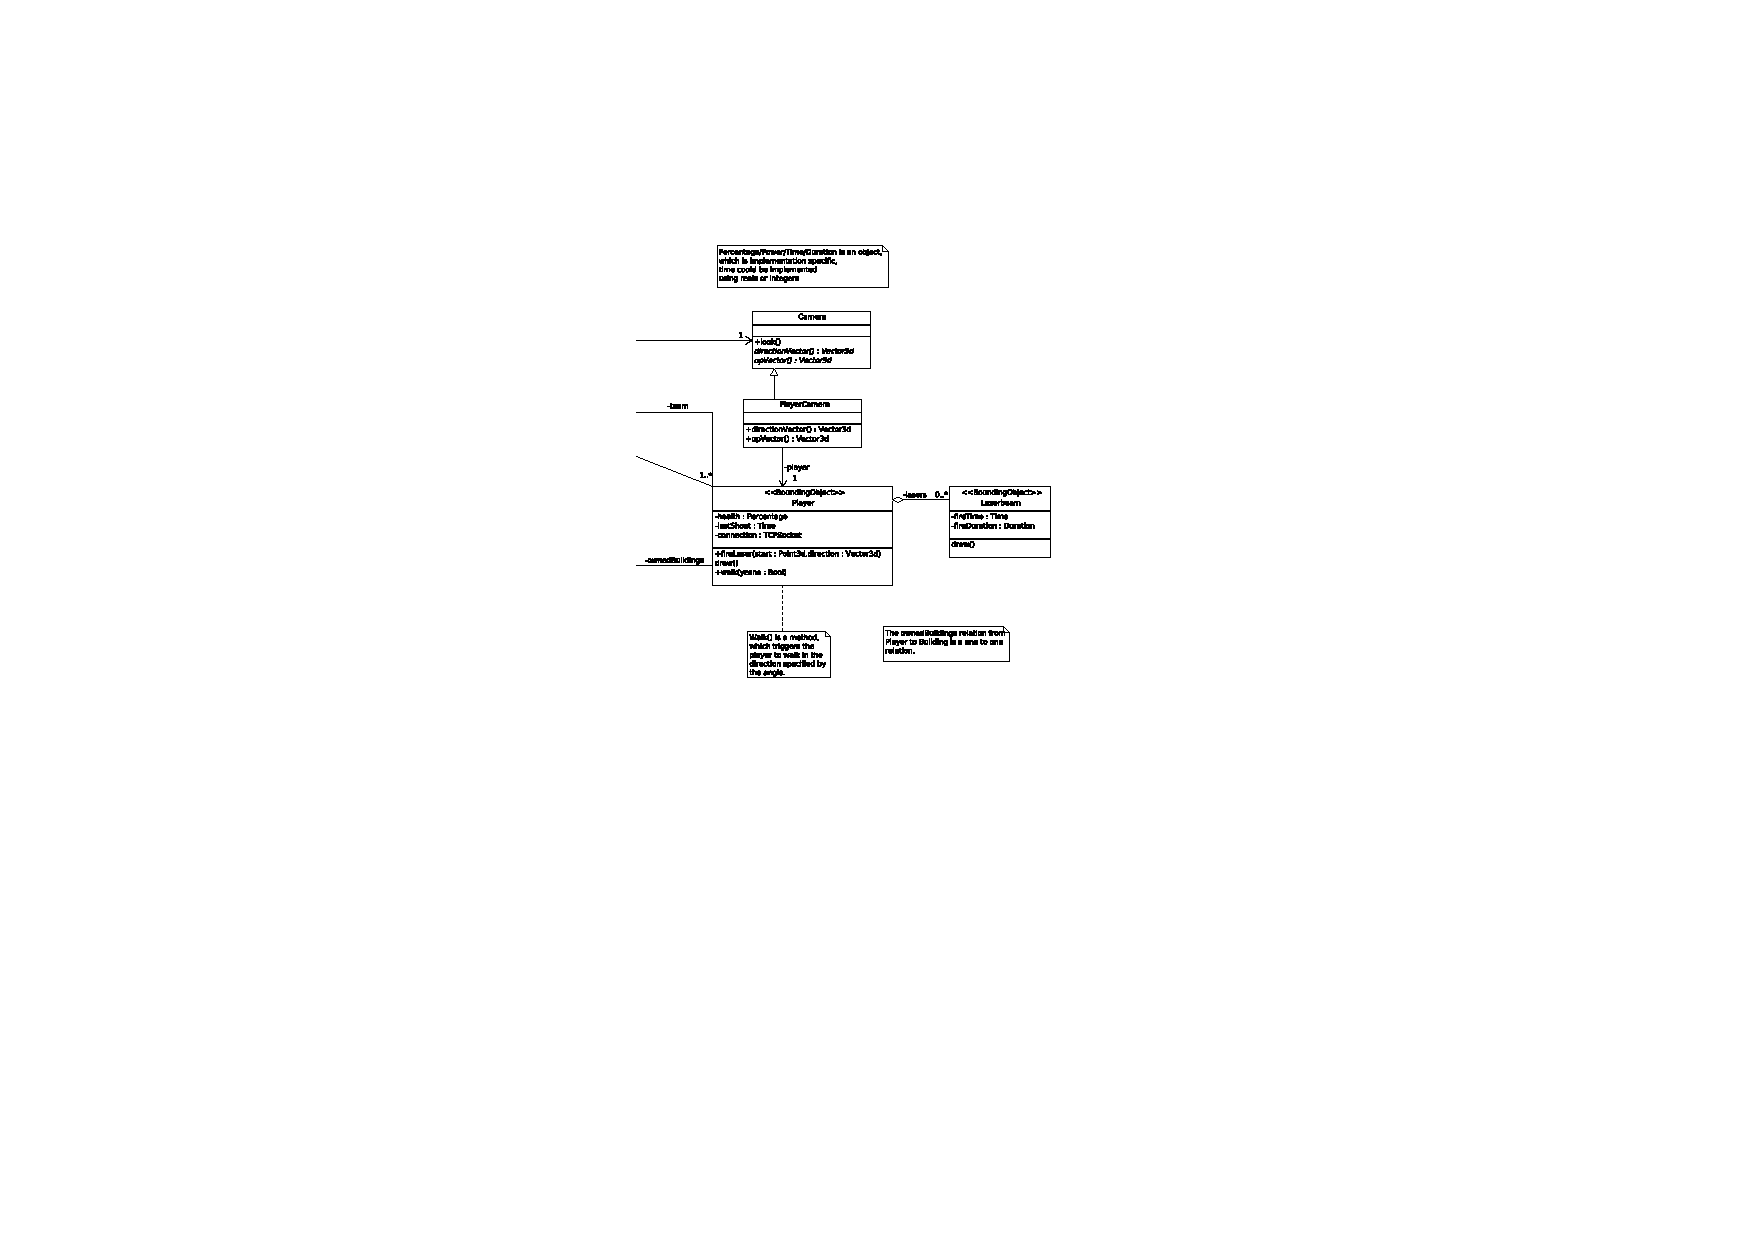
\includegraphics[height=0.6\textheight]{../Class-diagram/ClassDiagram2.pdf}
    \newpage
    
        \section{Het berichtsformaat}
    \label{app:berichtsformaat}
    We zijn nu klaar om het formaat van de berichten formeel te defini\"eren. Hiervoor gebruiken we BNF (\emph{Backus-Naur Form}):
	
	\begin{center} \boxed{\begin{aligned}
    <\textsc{message}> &::= <\textsc{command}> <\textsc{args}> <\textsc{crlf}> \\
    <\textsc{command}> &::= \text{``A''...``Z''} <\textsc{command}> | \text{``A''...``Z''} \\
    <\textsc{args}>    &::= \text{`` ''} | <\textsc{string}> | <\textsc{value}> <\textsc{args}> \\
    <\textsc{string}>  &::= \text{`` :''} <\text{printable characters}>^{*} \\
    <\textsc{value}>   &::= \text{`` ''}  <\text{graphical characters}>^{*} \\
    <\textsc{crlf}>    &::= \textsc{cr lf}
    \end{aligned} }\end{center}

    Een bericht bestaat uit een commando met argumenten. Na het commando en argumenten komt het einde van de regel: \textsc{crlf}. Met ``A''...``Z'' bedoelen we een willekeurige hoofdletter. Een commando is dus een hoofdletter of een hoofdletter gevolgd door een commando. Hieruit volgt dat een commando een niet-lege reeks van hoofdletters is.

    Het argument van een commando is alleen een spatie, een string of een waarde gevolgd door een argument. Een string begint altijd met een spatie gevolgd door een dubbele punt. Vervolgens volgt een willekeurige reeks van ``printable characters''. Hiermee bedoelen we letters, cijfers en spaties. Een waarde begint ook altijd met een spatie. Daarna volgt een reeks van ``graphical characters''. Daarmee bedoelen we letters en cijfers.

    We merken nog op dat het mogelijk is om een bericht te sturen zonder argumenten. Dit kan wel degelijk nuttig zijn, aangezien er bijvoorbeeld ook informatie kan worden gehaald uit het commando zelf.

    Het onderscheid tussen een value en een string is dus klein. Een string is altijd het laatste onderdeel van een argument. Merk op dat de verschillende argumenten worden onderscheiden door spaties. Aangezien er nog een dubbele punt voor de string staat, mag een string wel spaties bevatten zonder dat hierdoor onze berichten meerdere betekenissen krijgen. Immers, zodra we een spatie gevolgd door een dubbele punt tegenkomen, kunnen we concluderen dat we aan het laatste argument zijn begonnen. Een spatie is dan onderdeel van het argument zelf en betekent dus niet dat een nieuw argument is begonnen. Op deze manier kunnen namen van spelers en de naam van het spel spaties bevatten. 
    \newpage
    
        \section{De berichten}
    \label{app:berichten}
    We zullen nu alle gebruikte berichten afgaan met een korte toelichting. De berichten zullen natuurlijk voldoen aan het berichtsformaat zoals gespecificeerd in appendix \ref{app:berichtsformaat}. We zullen vooral kijken naar het nut voor de ontvanger. Om de berichten te beschrijven gebruiken we een aantal conventies. We zullen voor de leesbaarheid komma's plaatsen tussen de verschillende argumenten. Deze zijn dus niet deel van het bericht. Ook zullen we de commando's laten eindigen met een punt, dit moet dan worden gelezen als \textsc{cr lf}.

    \subsection{Server detectie}
    Het \emph{Broadcast} bericht wordt gebruikt voor het detecteren van servers tijdens de initialisatie. Dit bericht word periodiek door servers verstuurd met behulp van broadcast over \udp. We hebben ervoor gekozen om dit bericht elke vijf seconden te sturen. De wachttijd voor de gebruikers is dan nog steeds verwaarloosbaar, terwijl het netwerk nauwelijks wordt belast.

    Spelers moeten continu voor deze Broadcast berichten scannen. De gevonden servers worden dan in een lijst gezet. De speler kan dan uit deze lijst van servers kiezen. Hierdoor kunnen processen in hetzelfde subnet een server vinden. We geven ook de mogelijkheid om direct het ip van de server op te geven. Dit heeft het grote voordeel dat het mogelijk wordt om ook te spelen met spelers buiten het lokale netwerk. Merk op dat de server natuurlijk alleen wordt gebruikt voor het opzetten van het spel.

    Het bericht bevat de versie van het spel en het huidige aantal spelers. Bovendien bevat het de naam van het spel. Het bericht heeft de volgende syntax:
    \bericht{GOTO, version, numPlayers :gameName.}

    \subsection{De lobby}
    Het \emph{Name} bericht wordt gebruikt na de server detectie. Als een speler de lobby van een bepaald spel wil binnengaan, wordt dit gedaan door een Name bericht te sturen. In dit bericht aan de server stuurt de speler zijn gewenste naam mee:
    \bericht{NAME :playername.}
    Indien de speler wordt toegelaten, zal de server een \emph{Hello} bericht terugsturen als reactie op het Name bericht (en wordt dus alleen gestuurd aan de speler die het Name bericht heeft gestuurd aan de server). Hierin staat het toegewezen ID van de speler, de versie, het aantal spelers en de naam van het spel. Dit geeft het volgende bericht:
    \bericht{HELLO, pid, version, numPlayers :gameName.}
    Na het versturen van het Hello bericht, zal de server ook meteen een aantal \emph{Player} berichten sturen. Dit bericht wordt aan de nieuwe speler gestuurd om het team en status van elke medespeler kenbaar te maken. De status kan B zijn voor niet ready, R zijn voor ready of H zijn voor host. Alle spelers zitten standaard in hetzelfde team. Bovendien hebben alle spelers standaard de status niet ready. Het spel kan pas beginnen als alle spelers ready zijn. Dan kan de speler, die de server draait, op start drukken om het spel te starten. Het bericht heeft de volgende syntax:
    \bericht{PLAYER, pid, tid, state :playerName.}
    Na het versturen van de Hello en Player bericht, zal de server aan alle spelers een \emph{Join} bericht sturen. Hierdoor weten alle spelers dat er een nieuwe medespeler is bijgekomen. Dit bericht wordt ook aan de nieuwe speler zelf gestuurd. Hierdoor kan de nieuwe speler concluderen dat de Player berichten zijn afgelopen. Dit bericht bevat de ID van de speler en de naam van de speler:
    \bericht{JOIN, pid :playerName.}
    Het \emph{Part} bericht wordt gestuurd als de verbinding van een speler met de server, al dan niet vrijwillig, wordt verbroken. Dit bericht wordt aan iedereen gestuurd om mede te delen dat een van de medespelers is vertrokken. We sturen alleen de ID van de vertrokken speler mee:
    \bericht{PART, pid.}
    Met een \emph{Team request} bericht kan de speler een verzoek naar de server sturen om van team te wisselen. Dit bericht bevat dan het nieuwe gewenste team van de speler:
    \bericht{TEAM, tid.}
    Als een speler van team is gewisseld, wordt dit kenbaar gemaakt door de server met het \emph{Team} bericht. De server stuurt dan aan de andere spelers het volgende bericht om dit kenbaar te maken:
    \bericht{TEAM, pid, tid.}
    Verder zijn er nog \emph{Ready request} en \emph{Busy request} berichten. Een speler kan de ready en busy berichten gebruiken om zijn status te veranderen. Ready betekent dat de status ready moet worden, terwijl Busy betekent dat de status niet ready moet worden. Impliciet wordt er een afbeelding bijgehouden tussen het IP-adres, de speler ID en de naam van de speler. Dit geeft de volgende twee berichten:
	\bericht{READY.}
    \bericht{BUSY.}
    Nadat een speler van team is gewisseld, maakt de server dit kenbaar aan de andere spelers. Dit wordt gedaan door de ID van de speler mee te sturen:
    \bericht{READY, pid.}
    \bericht{BUSY, pid.}
    Een speler kan chatten met de andere spelers. Dit wordt gedaan door een \emph{Chat request} bericht te sturen naar de server. Dit bericht bevat dan het chatbericht:
    \bericht{CHAT :msg.}
    Zodra de server een Chat request bericht ontvangt, stuurt de server een \emph{Chat} bericht naar alle andere spelers. Dit bericht bevat de ID van de speler en het chatbericht:
    \bericht{CHAT, pid :msg.}
    Merk op dat er soms twee commando's zijn met dezelfde naam. Deze zijn echter zeer eenvoudig van elkaar te onderscheiden. In dit geval is er namelijk voor gezorgd dat \'e\'en commando alleen door de clients wordt verzonden en het andere commando alleen door de server. Hierdoor ontvangt elke speler nooit meer dan \'e\'en van de twee type commando's.

\subsection{Berichten om het spel op te zetten}
Om het spel op te kunnen zetten hebben we ook speciale berichten nodig. Met behulp van deze berichten proberen we een volledige graaf en een token ring op te bouwen. Met een \emph{Good-day} bericht maakt de speler contact met de server. Zo kan de speler toegevoegd worden aan de graaf. \textsc{tid} identificeert het team en \textsc{name} geeft de speler een naam.
\bericht{GOODDAY, tid :name.}

Nadat de server een \emph{Good-day} bericht heeft ontvangen, stuurt de server een \emph{Welcome} bericht als antwoord. \textsc{pid} wijst de speler een uniek ID toe. Version is een parameter om af te dwingen dat alle spelers de zelfde versie hebben. \textsc{iplist} is een string van alle IP-adressen in de standaard \textsc{cidr} notatie (dat wil zeggen dat een adres gerepresenteerd wordt in de vorm: \textsc{xxx.xxx.xxx.xxx}). Tussen elk IP-adres wordt het karakter \emph{e} gebruikt om IP-adressen te onderscheiden.
\bericht{WELCOME, pid , version :iplist.}

Het \emph{Sup} bericht wordt gestuurd door een speler zodra hij een verbinding met een andere speler aanmaakt. \textsc{pid} geeft de speler ID van de speler die het bericht verstuurt aan en \textsc{version} zorgt er weer voor dat de versies overeenkomen. \textsc{name} geeft de naam van de speler aan.
\bericht{SUP, pid, version :name.}

Het \emph{Gladtomeetyou} bericht is een bevestiging van het \emph{Sup} bericht. Hiermee geeft de speler, welke het \emph{Sup} bericht ontving, aan wat zijn naam en speler ID is. \textsc{pid} is dan weer de speler ID en name de naam van de speler.
\bericht{GLADTOMEETYOU, pid :name}

\subsection{Berichten tijdens het spel}
De volgende berichten worden gebruikt voor communicatie tijdens het spel. Deze berichten worden dan naar alle andere spelers gestuurd. Sommige berichten zijn hierbij aangegeven met een R. Deze berichten krijgen een speciale behandeling, zoals wordt besproken in sectie \ref{sec:tijdensspel}. Als eerste is er een zogenaamd \emph{GameChat} bericht. Dit bericht vervult een vergelijkbare taak als het Chat bericht in de lobby. Het GameChat bericht heeft de volgende syntax:
\bericht{GAMECHAT, message.}

Een speler zal periodiek zijn huidige positie doorsturen. Bovendien wordt hierbij de huidige richting meegegeven. Hiervoor wordt het \emph{Move} bericht verstuurd:
\bericht{MOVE, x, y, z, vx, vy, vz.}

Als een speler heeft geschoten, dan wordt dit naar alle andere spelers gestuurd. Hierbij wordt de oorsprong van het schot en de richting van het schot meegestuurd. Merk op dat deze overeenkomen met respectievelijk de positie van de speler en de kijkrichting. De bedoeling van dit bericht is enkel om de bijbehorende animatie weer te geven: eventuele schade aan het harnas wordt apart afgehandeld.
\bericht{FIRE, x, y, z, vx, vy, vz.}

De spelers houden lokaal de totale hoeveelheid goud van het team bij. Spelers zullen deze waarde periodiek versturen. Als deze waarden tussen verschillende spelers van hetzelfde team niet overeenkomen, zullen we deze waarden middelen. Het bericht \emph{Team} verstuurt de ID van het team en de hoeveelheid goud:
\bericht{TEAM, tid, teamGold.}

Verder is er nog een \emph{Respawn} bericht. Dit bericht wordt verstuurd nadat een speler is dood gegaan. In dit bericht wordt de nieuwe locatie meegestuurd, dit zal in principe het commandocentrum van het bijbehorende team zijn:
\bericht{R RESPAWN, x, y, z.}

Na een schot zal een speler berekenen of een speler van het andere team is geraakt. Als dit het geval is, dan zal de geraakte speler en de hoeveelheid schade worden verstuurd. Merk op dat dit lokaal wordt berekend. Het hoeft niet noodzakelijk te zijn dat het schot van de speler zelf komt, het kan ook komen van een gebouw in het bezit van een speler. De geraakte speler en de hoeveelheid schade wordt doorgegeven in het bericht \emph{Hit}:
\bericht{R HIT, pid, damage.}

Als een speler is doodgegaan, zal hij dit kenbaar maken aan alle andere spelers. Dit wordt gedaan door het \emph{Died} bericht, waarin ook de dader is opgenomen. Op zich is de informatie over de dader irrelevant voor het spel, maar dit kan wel worden gebruikt om het spel verder uit te breiden.
\bericht{R DIED, pid.}

Een speler zal een voorwerp achterlaten bij het doodgaan. In het huidige ontwerp zal dit altijd een muntje zijn. Dit muntje krijgt meteen ook een unieke ID en een zekere waarde. Verder zal nog de lokatie van het muntje worden meegestuurd. Als laatste zal nog het type voorwerp worden meegestuurd, dit argument kan worden gebruikt voor verdere uitbreiding. Samen geeft dit het \emph{Drop} bericht:
\bericht{R DROP, id, x, y, z, value, type.}

Als een speler een voorwerp opraapt, zal er een \emph{Take} bericht worden verstuurd. Hierbij zal natuurlijk ook de ID van het opgeraapte voorwerp worden meegestuurd.
\bericht{R TAKE, id.}

Een speler kan natuurlijk ook een gebouw bouwen. Het spel heeft de lokale verantwoordelijkheid om te controleren dat de bouwplaats toegestaan is. In het \emph{Build} bericht wordt naast de lokatie ook nog een uniek ID en het type van het gebouw meegestuurd:
\bericht{R BUILD, id, x, y, z, type.}

Als een speler een gebouw heeft geraakt met een schot, dan zal de ID van het gebouw worden verstuurd en de hoeveelheid schade. Dit wordt gedaan in het \emph{Attack} bericht:
\bericht{R ATTACK, id, damage.}

Op een gegeven moment kan het ook gebeuren dat het gebouw is vernietigd. De eigenaar van het gebouw heeft de verantwoordelijkheid om dit te controleren. Als het gebouw is vernietigd, dan wordt de ID van het gebouw verstuurd. Bovendien zal de dader hierbij worden verstuurd net zoals in het geval dat een speler is doodgegaan. Hiertoe wordt het \emph{Destroy} bericht gebruikt:
\bericht{R DESTROY, id, pid.}

Als laatste is er nog het \emph{End} bericht. Dit bericht wordt verstuurd zodra een team heeft gewonnen: oftewel als het commandocentrum van het andere team is vernietigd. In dit bericht wordt het winnende team meegestuurd:
\bericht{R END, tid.} 
    \newpage
    
    \section{Voorbeeld van de interactie tussen de gebruikersomgeving en de protocolmodule}
    \label{sec:interactscenmodel}
    \begin{figure}[h]
    	\centering
	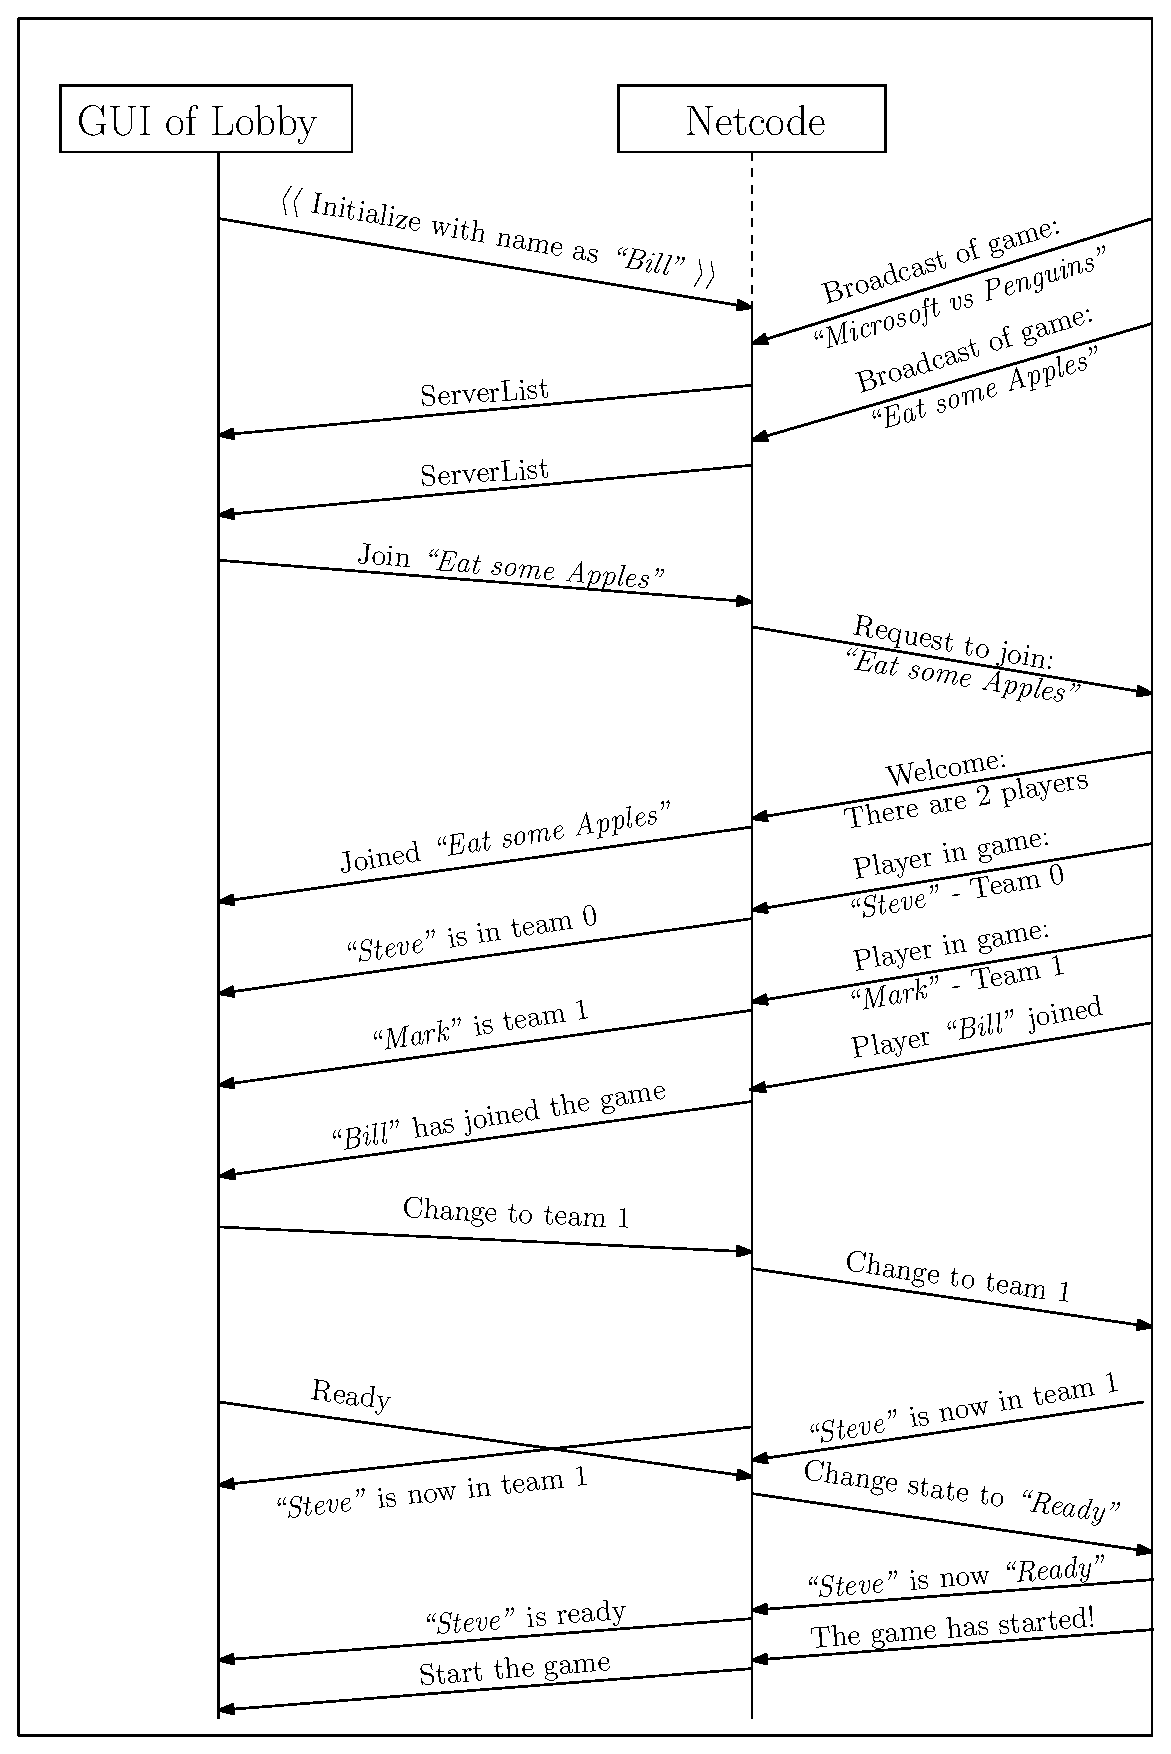
\includegraphics[height=0.7\textheight]{../Class-diagram/MSCLobby-console.eps}
	\caption{Voorbeeld van een interactie van de gebruikersomgeving en de protocolmodule.}
    \end{figure}
    \label{app:MSCLobbyCon}
       
%    Andere appendices
%    Invoegen gaat nog erg slecht
%    \section{Verslag werkplan}
%    \documentclass[a4paper,11pt]{article}
\usepackage{graphicx,listings,float,geometry}
%\usepackage[firstpage]{draftwatermark}
%\SetWatermarkLightness{0.5}
%\SetWatermarkScale{4}
\setcounter{tocdepth}{2}

\geometry{
	includeheadfoot,
	margin=2.54cm
}

\newcommand{\BS}{BrnStrm}
\newcommand{\ON}{Ori\"entatie}
\newcommand{\MW}{Werkplan}
\newcommand{\MS}{SpelSpec}
\newcommand{\MA}{Spelkeus}
\newcommand{\BO}{Deel. Docu.}
\newcommand{\OC}{Protocol}
\newcommand{\MN}{Impl.Proto.}
\newcommand{\CT}{Proto Test}
\newcommand{\MK}{Klas.diagr.}
\newcommand{\MT}{Taakverdel.}
\newcommand{\IS}{Implement}
\newcommand{\BG}{Handl.}
\newcommand{\AV}{Eind Docu}
\newcommand{\ME}{Mkn.prsnt.}
\newcommand{\EP}{Presenteren}

\usepackage[dutch]{babel}
\newenvironment{widepar}%
  {\setlength{\leftskip}{-\marginparsep}\addtolength{\leftskip}{-\marginparwidth}}{\par}

\begin{document}
	\begin{titlepage}
	\begin{center}
		
		{\Huge Informele Specificatie \\[0.5cm]OGO 2.3 - Multiplayer Game}\\[0.5cm]
		\rule{\linewidth}{0.5mm}\\[0.5cm]
				\bigskip
		\huge \textit{``Grudge of the Oblivious''}
		
		{\Large
		Luca van Ballegooijen, Tim van Dalen, \\
		Carl van Dueren den Hollander, Peter Koymans,\\
		Kay Lukas en Ferry Timmers\\[1cm]
		}
		
		{\large
		OGO 2.3\\
		Groep 3 \\[1cm]
		Faculteit Wiskunde en Informatica\\
		Technische Universiteit Eindhoven\\[1cm]
		}
		
		\begin{abstract}

    In dit document zullen we de kritieke punten bij dit project identificeren. Vervolgens bekijken we de taken die bij dit project een rol spelen. Tenslotte zullen we dit gebruiken om een werkplan voor het project op te stellen.
\end{abstract}


		\vfill

		{\large \today}
	\end{center}
\end{titlepage}

	
	\tableofcontents
	\newpage

	\section{Kritieke punten}
    We beginnen met het identificeren van de kritieke punten. Met deze kritieke punten kan dan later rekening worden gehouden in het werkplan. De voornaamste problemen tijdens dit project zijn:
    \begin{enumerate}
    \item[(a)] Het grootste probleem voor het maken van het programma is het netwerk aspect. Hierbij identificeren we twee mogelijke obstakels. Ten eerste moet het mogelijk zijn om elkaar te kunnen vinden over het netwerk. Dit is zeker geen triviale taak. Ten tweede geldt dat gedurende het spel alle machines op gelijke voet staan. Er mag dus geen server worden gebruikt, wat het ontwerp van het spel moeilijker maakt.
    \item[(b)] Een ander groot gevaar is complexiteit. Bij het ontwikkelen van een spel kan men al snel uit enthousiasme hoge verwachtingen krijgen en hoge eisen stellen. Deze overmaat aan eisen kan later te veel werk blijken.
    \item[(c)] Een laatste hindernis is het gedistribueerde aspect met name in conflictsituaties. Een goed voorbeeld hiervan is als twee spelers op hetzelfde moment voedsel proberen te pakken. Als hier geen rekening mee wordt gehouden, kan dit leiden tot een inconsistente toestand. Zo zou het kunnen gebeuren dat beide spelers \'e\'en voedsel object verkrijgen, wat ongewenst is.
    \end{enumerate}

    In ons werkplan proberen we al vroeg mogelijk om met deze kritieke punten rekening te houden. Aangezien we (a) als het voornaamste probleem beschouwen, zullen we in week 1 ons al ori\"enteren op het probleem. We zullen vooral kijken naar de mogelijkheden voor broadcast. Probleem (b) pakken we aan door te beginnen met een kleine hoeveelheid aan eisen voor het spel. Later kan het spel dan worden uitgebreid. In verband met probleem (c) is het slim om al snel te beginnen met het ontwerp van het communicatieprotocol. Er wordt pas begonnen aan dit aspect van het programma zodra het communicatieprotocol is voltooid. Na het voltooien van het communicatieprotocol zal dit uitgebreid worden getest.

    \section{De taken}
    Nu we de mogelijke problemen hebben bekeken, zijn we klaar om een lijst met taken op te stellen met afkortingen. De genoemde taken staan ruwweg in chronologische volgorde:
    \begin{enumerate}
    \item[-] Brainstormen over spelidee (\emph{\BS}).
    \item[-] Ori\"entatie op netwerk aspect door het maken van eenvoudig chat programma (\emph{\ON}).
    \item[-] Maken werkplan met taakverdeling (\emph{\MW}).
    \item[-] Maken spelspecificatie en gebruikershandleiding (\emph{\MS}).
    \item[-] Maken alternatieven en motivering van spelkeuze (\emph{\MA}).
    \item[-] Beschrijving onderdelen en onderlinge samenhang (\emph{\BO}).
    \item[-] Ontwerpen communicatieprotocol (\emph{\OC}).
    \item[-] Maken onderliggende netwerkcommunicatie (\emph{\MN}).
    \item[-] Communicatieprotocol testen (\emph{\CT}).
    \item[-] Maken klassendiagram (\emph{\MK}).
    \item[-] Maken taakverdeling voor implementatie (\emph{\MT}).
    \item[-] Implementatie spel (\emph{\IS}).
    \item[-] Bijwerken gebruikershandleiding, validatie aannames en motivering implementatie (\emph{\BG}).
    \item[-] Afronden verslag (\emph{\AV}).
    \item[-] Maken eindpresentatie (\emph{\ME}).
    \item[-] Eindpresentatie (\emph{\EP}).
    \end{enumerate}

    \section{Het werkplan}
    Als laatste moeten de taken nog over de personen worden verdeeld. Hierbij zullen we taken proberen te rouleren zodanig dat iedereen zowel taken heeft voor programmeren als documenteren. Aangezien wij allemaal zowel ervaring hebben met programmeren als met documenteren, zullen we bij de taakverdeling geen speciale rekening houden met de koppels (bijvoorbeeld relatief goede programmeurs bij relatief zwakke programmeurs).

    We hebben besloten om drie belangrijke zaken samen te doen. Ten eerste is het natuurlijk erg logisch dat het brainstormen samen gebeurt. Hierdoor weten we allemaal in welke richting het spel zal gaan, wat bij alle volgende stappen van belang zal zijn. Ten tweede wordt het communicatieprotocol samen ontworpen. Dit heeft tot doel zodat iedereen het communicatieprotocol goed snapt, zodat iedereen hiermee overweg kan met de implementatie. Ten derde wordt het testen van het communicatieprotocol samen gedaan. De voornaamste reden hiervoor is vanwege de grote diversiteit aan operating systemen in onze groep, wat eventueel problemen kan geven bij de implementatie. We zijn nu klaar om het volledige werkplan te geven, we gebruiken hierbij de eerder gegeven afkortingen. De deadlines staan op een aparte regel en zijn schuin gedrukt:
        \begin{figure}[H]
        \small
        \centering
        \begin{tabular}{| l | l | l | l | l | l | l |}
        \hline
        Week & Carl & Ferry & Kay & Luca & Peter & Tim \\ \hline
        Week 1 24-04-2012 & \BS & \BS & \BS & \BS & \BS & \BS \\ \hline
        Week 1 25-04-2012 & \ON & \ON & \ON & \ON & \MW & \ON \\ \hline
        Week 1 26-04-2012 & \ON & \ON & \ON & \ON & \MW & \ON \\ \hline
        Week 2 01-05-2012 & \MS & \MA & \MA & \MS & \MA & \MS \\ \hline
        Week 2 02-05-2012 & \MS & \MA & \MA & \MS & \MA & \MS \\ \hline
        Week 2 03-05-2012 & \MS & \MA & \MA & \MS & \MA & \MS \\ \hline
        Week 2 04-05-2012 & \multicolumn{6}{|c|}{\emph{Deadline ori\"entatiefase}} \\ \hline
        Week 3 08-05-2012 & \MS & \MA & \MA & \MS & \MA & \MS \\ \hline
        Week 3 09-05-2012 & \MS & \MA & \MA & \MS & \MA & \MS \\ \hline
        Week 3 10-05-2012 & \MS & \MA & \MA & \MS & \MA & \MS \\ \hline
        Week 4 15-05-2012 & \OC & \OC & \OC & \OC & \OC & \OC \\ \hline
        Week 4 16-05-2012 & \OC & \OC & \OC & \OC & \OC & \OC \\ \hline
        Week 4 16-05-2012 & \multicolumn{6}{|c|}{\emph{Deadline specificatiefase}} \\ \hline
        Week 5 22-05-2012 & \BO & \MN & \MK & \MK & \BO & \MN \\ \hline
        Week 5 23-05-2012 & \BO & \MN & \MK & \MK & \BO & \MN \\ \hline
        Week 5 24-05-2012 & \BO & \MN & \MK & \MT & \BO & \MN \\ \hline
        Week 6 30-05-2012 & \BO & \MN & \MK & \MT & \BO & \MN \\ \hline
        Week 6 31-05-2012 & \CT & \CT & \CT & \CT & \CT & \CT \\ \hline
        Week 6 01-06-2012 & \multicolumn{6}{|c|}{\emph{Deadline ontwerpfase}} \\ \hline
        Week 7 05-06-2012 & \IS & \IS & \IS & \IS & \IS & \IS \\ \hline
        Week 7 06-06-2012 & \IS & \IS & \IS & \IS & \IS & \IS \\ \hline
        Week 7 07-06-2012 & \IS & \IS & \IS & \IS & \IS & \IS \\ \hline
        Week 8 12-06-2012 & \BG & \IS & \IS & \IS & \IS & \BG \\ \hline
        Week 8 13-06-2012 & \BG & \IS & \IS & \IS & \IS & \BG \\ \hline
        Week 8 14-06-2012 & \BG & \IS & \IS & \IS & \IS & \BG \\ \hline
        Week 8 14-06-2012 & \multicolumn{6}{|c|}{\emph{Deadline implementatiefase eerste versie}} \\ \hline
        Week 9 19-06-2012 & \AV & \AV & \ME & \AV & \AV & \ME \\ \hline
        Week 9 20-06-2012 & \AV & \AV & \ME & \AV & \AV & \ME \\ \hline
        Week 9 21-06-2012 & \EP & \EP & \EP & \EP & \EP & \EP \\ \hline
        Week 9 22-06-2012 & \multicolumn{6}{|c|}{\emph{Deadline verslag}} \\ \hline
        \end{tabular}
        \caption{Gedetailleerde taakverdeling per dag}
        \label{tab:planning}
    \end{figure}

    Zoals in de tabel is te zien, zijn er ongeveer twee weken om aan de implementatie te werken. Het idee is dat dan een groot deel van het netwerk aspect, wat het grootste risico heeft om uit te lopen, daarvoor al af te hebben om dit op te vangen. Bij de implementatie moet dus vooral aandacht worden besteed aan het modelleren van de scene en het maken van het spel. Een gedetailleerde beschrijving voor de taakverdeling wordt pas in week 6 gemaakt, aangezien daarvoor een deel van de ontwerpfase al moet zijn voltooid.
\end{document}

%    \includepdf[pages={-}]{../../werkplan/werkplan.pdf}
%    \newpage
%
%    \section{Verslag specificatie}
%    \includepdf[pages={-}]{../documentation.pdf}
%    \newpage
%
%    \section{Verslag alternatieven}
%    \includepdf[pages={-}]{../../keuze/documentation.pdf}
%    \newpage
%
%    \section{Verslag ontwerp}
%    \includepdf[pages={-}]{../Design/report.pdf}
%    \newpage
\end{document} 